% Written by Claude (2026-11-16): NN lecture on text and transformers. The
% slides are shared with NNDS (text-embeddings.tex from the CNN deck,
% transformers.tex from Lecture_transformers.tex); \NNDSorNN in those files
% holds the NN wording.
\documentclass[xcolor=x11names,compress,10pt,unknownkeysallowed,aspectratio=169]{beamer}
\usetheme{NN26}
% NN content helpers. The NN26 theme remains the presentation authority.
% Shared content style for NN and NNDS. Written by Claude (2026-10-14).
%
% Everything that shared slides rely on lives here, loaded by both courses:
% colors, notation helpers and the card system. Course themes own only the
% presentation around the content (header, footer, title page, fonts, the
% \myalert color and where \SlideSource text goes). Change a definition here,
% never by redefining it in a course file, so the two courses cannot drift.

\usepackage{mathtools,amssymb,tcolorbox}
\tcbsetforeverylayer{autoparskip}

% Semantic colors
\definecolor{darkred}{rgb}{0.55,0,0}
\definecolor{darkpastelblue}{rgb}{0.47,0.62,0.8}
\definecolor{darkcerulean}{rgb}{0.03,0.27,0.49}
\definecolor{darkgreen}{rgb}{0,0.55,0}

% Figure palette (draw.io defaults)
\definecolor{titlecolor}{RGB}{245, 242, 238}
\definecolor{drawgray}{HTML}{666666}
\definecolor{drawgray_l}{HTML}{F5F5F5}
\definecolor{drawblue}{HTML}{6C8EBF}
\definecolor{drawblue_l}{HTML}{DAE8FC}
\definecolor{drawgreen}{HTML}{82B366}
\definecolor{drawgreen_l}{HTML}{D5E8D4}
\definecolor{draworange}{HTML}{D79B00}
\definecolor{draworange_l}{HTML}{FFE6CC}
\definecolor{drawyellow}{HTML}{D6B656}
\definecolor{drawyellow_l}{HTML}{FFF2CC}
\definecolor{drawred}{HTML}{B85450}
\definecolor{drawred_l}{HTML}{EA6B66}
\definecolor{drawviolet}{HTML}{9673A6}
\definecolor{drawviolet_l}{HTML}{E1D5E7}

% Notation
\newcommand{\vc}[1]{\boldsymbol{\mathbf{#1}}}
\DeclareMathOperator*{\argmax}{arg\,max}
\DeclareMathOperator*{\argmin}{arg\,min}

% Cards: blue for definitions and computable quantities, green for goals and
% stable formulations, orange for warnings and trade-offs, red for
% training-specific or problematic elements.
\tcbset{
	nndsblue/.style={colback=drawblue_l!35!white,colframe=drawblue,boxrule=0.8pt,arc=1mm},
	nndsgreen/.style={colback=drawgreen_l!35!white,colframe=drawgreen,boxrule=0.8pt,arc=1mm},
	nndsorange/.style={colback=draworange_l!35!white,colframe=draworange,boxrule=0.8pt,arc=1mm},
	nndsred/.style={colback=drawred_l!12!white,colframe=drawred,boxrule=0.8pt,arc=1mm}
}

% A card that opens with \[ would start with an empty paragraph line plus the
% display skip, leaving more room above than below (by an amount that differs
% between engines). Set that leading equation as a centered display-style line
% instead, so the space above it is the card padding, as below.
\makeatletter
\newcommand{\nndscardlead}{\futurelet\nndscard@next\nndscard@check}
% tcolorbox follows this hook with \ignorespaces; look past it.
\def\nndscard@check{\ifx\nndscard@next\ignorespaces
	\expandafter\nndscard@skip\else\expandafter\nndscard@test\fi}
\def\nndscard@skip\ignorespaces{\nndscard@test}
\newcommand{\nndscard@test}{\@ifnextchar\[{\nndscard@display}{}}
\def\nndscard@display\[#1\]{{\centering$\displaystyle#1$\par}\@ifnextchar\end{}{\vspace{\belowdisplayskip}}}
\makeatother

% Card text is ragged-right: narrow justified columns open wide word gaps,
% especially in NNDS, which never hyphenates. Fixed display spacing: when
% parallel cards share a height, stretchable skips would otherwise spread
% the content unevenly.
\tcbset{
	nndscard/.style={before upper={\raggedright
		\setlength{\abovedisplayskip}{6pt}\setlength{\belowdisplayskip}{6pt}%
		\setlength{\abovedisplayshortskip}{6pt}\setlength{\belowdisplayshortskip}{6pt}%
		\nndscardlead}},
	nndsblue/.append style={nndscard},
	nndsgreen/.append style={nndscard},
	nndsorange/.append style={nndscard},
	nndsred/.append style={nndscard}
}

% Parallel cards share a group name and get equal heights; the second argument
% (a fixed height used by older NNDS slides) is ignored.
\tcbset{courseheight/.style 2 args={equal height group=#1}}

\usepackage{tikz}

% Matrix shapes written under a symbol, e.g. \shape{\vc{Q}}{(T,D_k)}.
\usepackage{stackengine}
\stackMath
\def\sss{\scriptstyle \color{gray}}
\setstackgap{L}{12pt}
\def\stacktype{L}
\newcommand{\shape}[2]{\stackunder{#1}{\sss #2}}

% Transformer slides: colors and diagram styles (moved here from the NNDS
% transformers-settings.tex on 2026-11-16, when NN adopted the lecture).

% Query, key and value colors, reused in equations and figures.
\colorlet{qcolor}{drawviolet!80!black}
\colorlet{kcolor}{draworange!85!black}
\colorlet{vcolor}{darkcerulean}
\newcommand{\qc}[1]{{\color{qcolor}#1}}
\newcommand{\kc}[1]{{\color{kcolor}#1}}
\newcommand{\vcl}[1]{{\color{vcolor}#1}}

% Block-diagram styles, as in shared/slides/mlps.tex and the deeper-models deck.
\tikzset{
    nnblock/.style={
            draw=drawblue, fill=drawblue_l!25!white, rounded corners=2pt,
            minimum width=1.25cm, minimum height=0.65cm,
            inner sep=5pt, font=\small
        },
    nnother/.style={nnblock, draw=drawgreen, fill=drawgreen_l!25!white},
    nnmerge/.style={
            circle, draw=drawgray, fill=white,
            minimum size=0.55cm, inner sep=1pt, font=\small
        },
    nnedge/.style={->, thick, draw=drawgray}
}

% Full-size diagram styles for the transformer figures: arrows as in the
% attention figures (Stealth tips, gray), boxes at normal size.
\tikzset{
    tfarr/.style={-{Stealth[length=5pt]}, drawgray, line width=0.6pt},
    tfblk/.style={draw=drawblue, fill=drawblue_l!60, rounded corners=2pt,
            minimum height=0.75cm, minimum width=1.9cm, inner sep=4pt, font=\small},
    tfnorm/.style={tfblk, draw=drawgreen, fill=drawgreen_l!70},
    tfsum/.style={circle, draw=drawgray, fill=white, minimum size=0.45cm, inner sep=0pt, font=\small},
    tflab/.style={font=\scriptsize, text=black!60},
}

\usetikzlibrary{positioning,arrows.meta,calc}
\newcommand{\myalert}[1]{{\color{redSap}\textbf{#1}}}
\newenvironment{whiteframe}[1]{\begin{frame}{#1}}{\end{frame}}
\newcommand{\eqnmarkbox}[3][]{#3}
\newcommand{\annotate}[4][]{}
\graphicspath{{./images/}{../upstream/nnds/latex/}}
\hypersetup{pdfauthor={Danilo Comminiello and Simone Scardapane}}

% Slide sources: bottom of the content area (the footline holds course details).
\providecommand{\SlideSource}[1]{\par\vfill{\scriptsize\color{drawgray}#1\par}}

% Shared transformer and text slides (Claude, 2026-11-16). NN text of the
% course switch, conventional subscripts for \idx, and code blocks in the NN26
% listings style (at the NNDS code size).
\newcommand{\NNDSorNN}[2]{#2}
\newcommand{\idx}[2]{{#1}_{#2}}
\lstnewenvironment{python}[1][]{\lstset{basicstyle=\ttfamily\footnotesize,columns=fullflexible,#1}}{}
\newcommand\pythoninline[1]{\lstinline[basicstyle=\ttfamily]!#1!}

\usetikzlibrary{decorations.pathreplacing}
% Real equation annotations instead of the NN stubs in nn-content.tex.
\let\eqnmarkbox\undefined
\let\annotate\undefined
\usepackage{annotate-equations}
\title{Tokens, embeddings and transformers}
\author[D. Comminiello \& S. Scardapane]{Danilo Comminiello and Simone Scardapane}
\date{}
\graphicspath{{assets/}{../../shared/assets/}}
\begin{document}
{\usebackgroundtemplate{
    \vbox to \paperheight{\hbox to \paperwidth{\hfil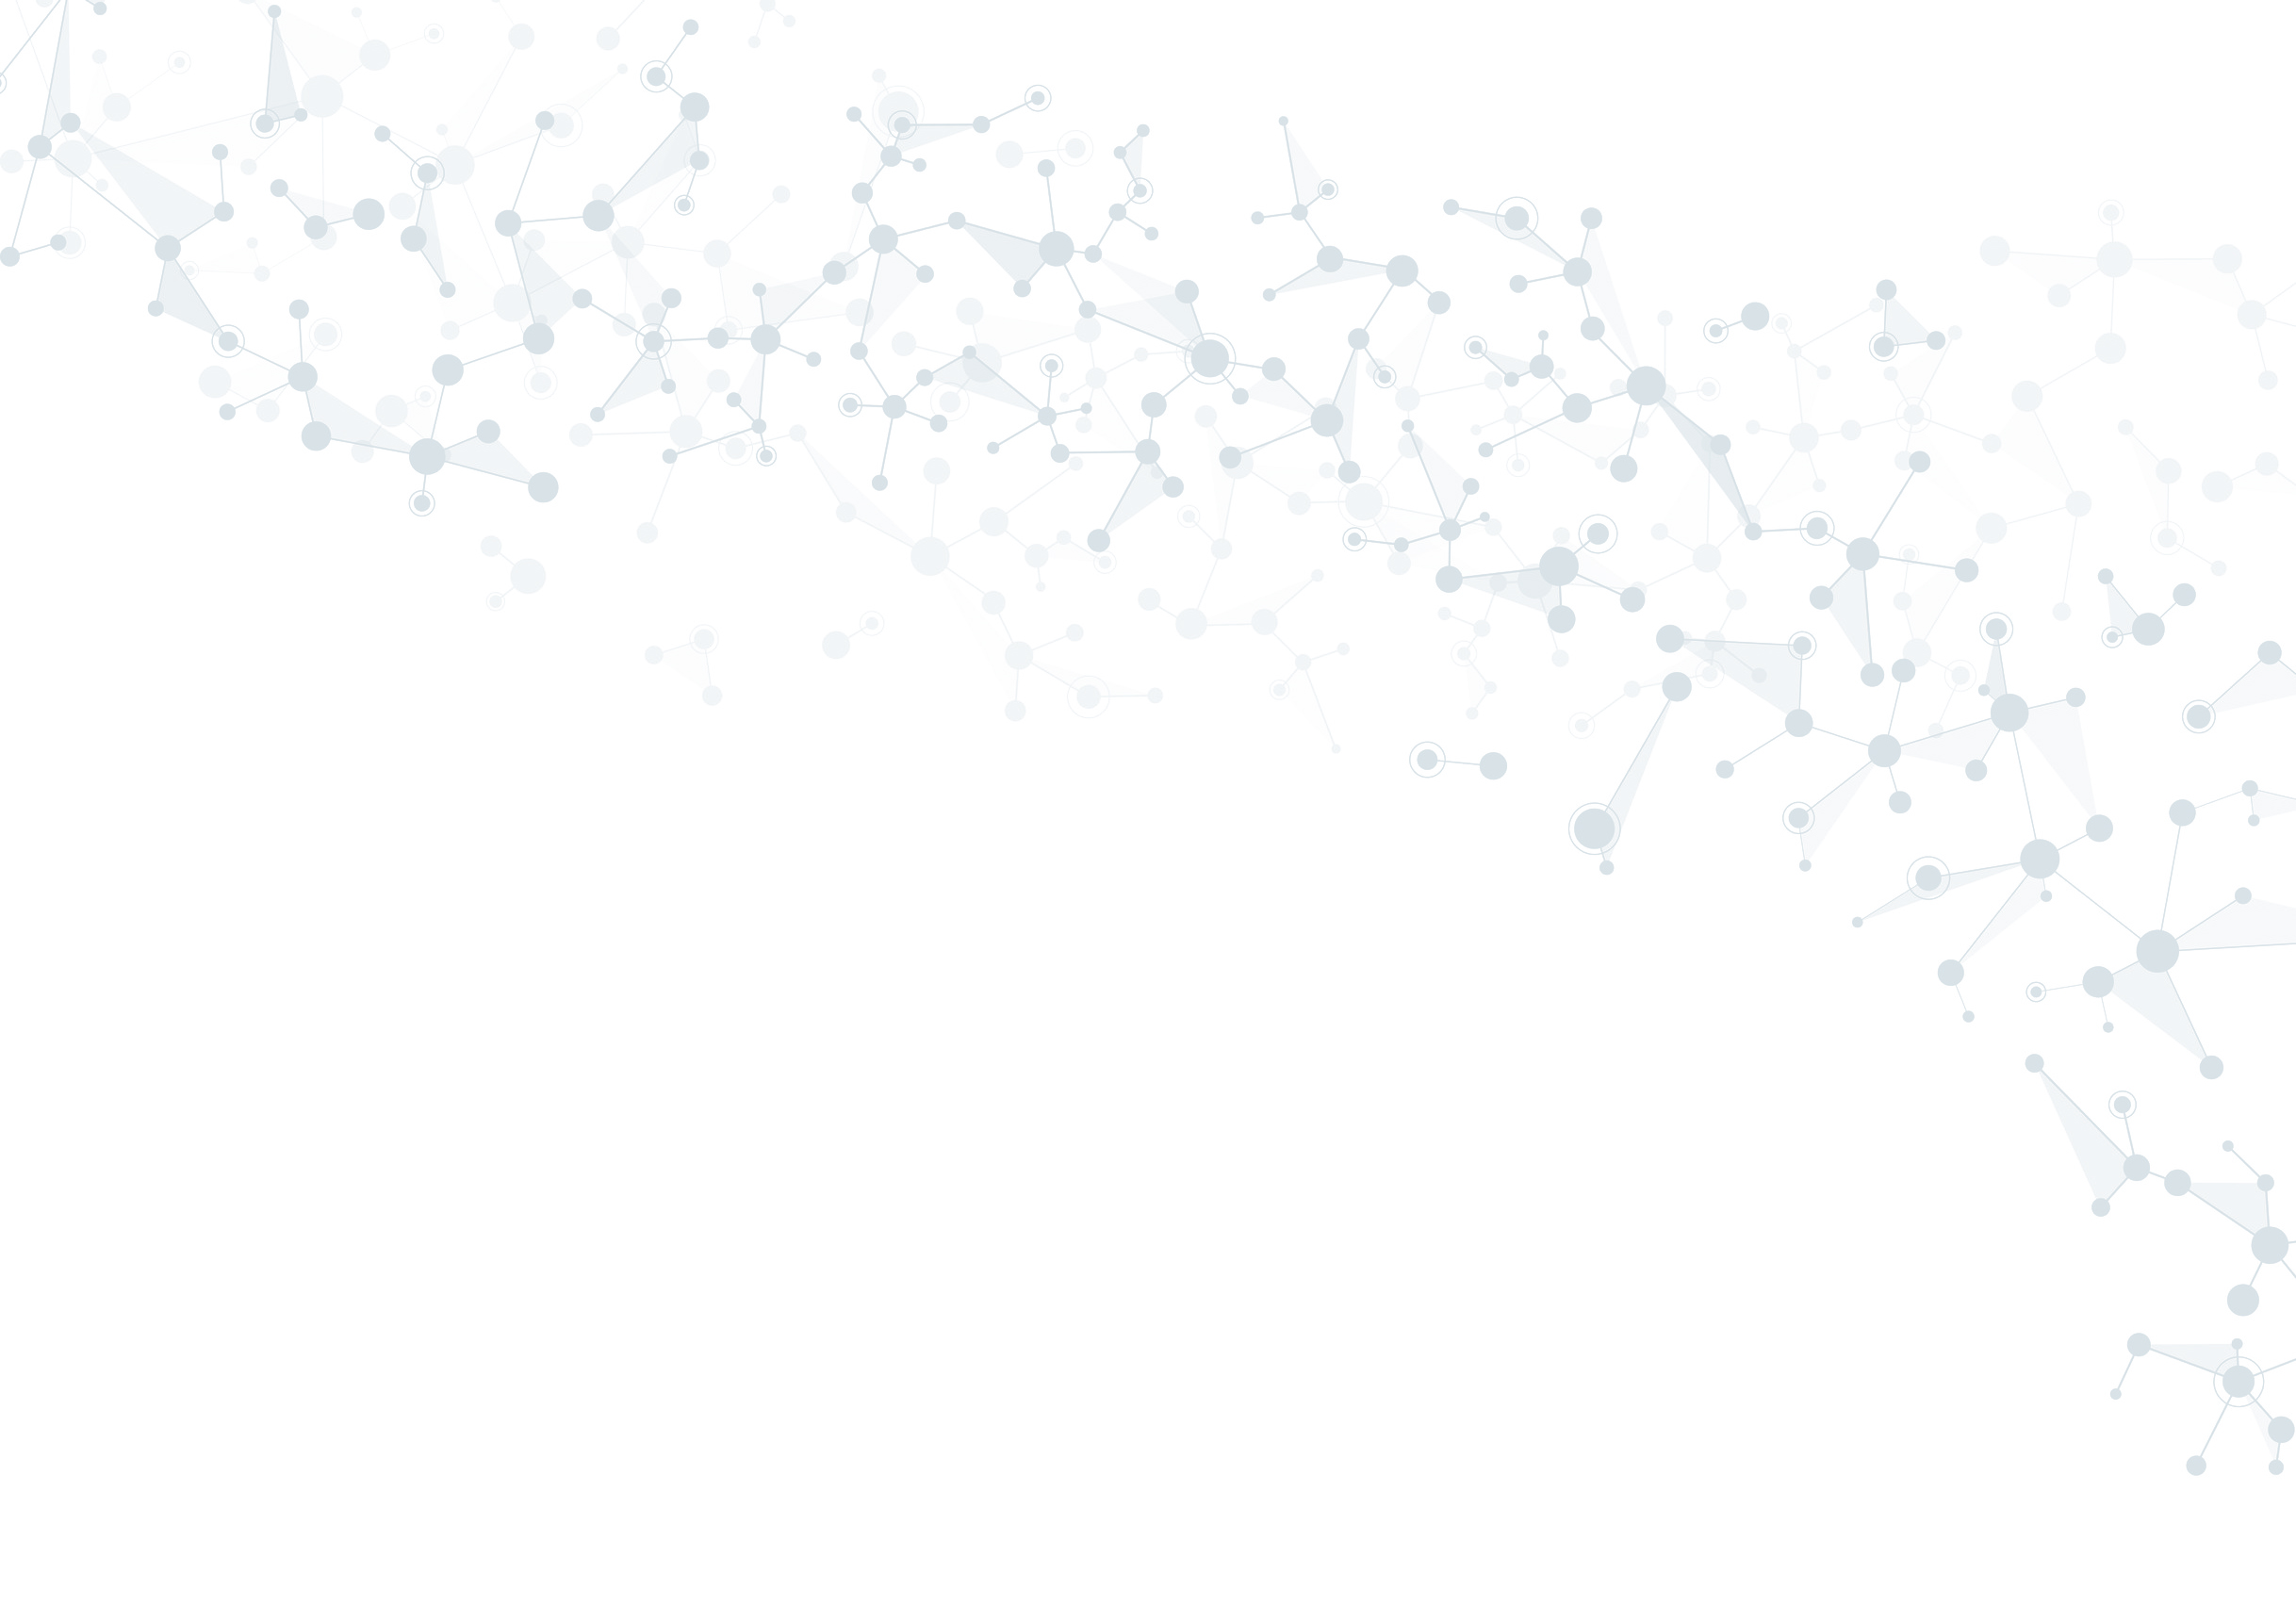
\includegraphics[keepaspectratio,width=\textwidth]{cover.jpg}\hfil}\vfil}}
\frame[plain]{\titlepage}}

\section{From text to embeddings}
% Text tokenization and embeddings, shared by the NNDS CNN deck and the NN
% transformer deck. Moved from Lecture_CNNs.tex by Claude (2026-11-16).

% Text pipeline rewritten step by step at Simone's request (2026-10-30), with
% new figures in shared/assets/images/text/{text_pipeline,tokenization,vocabulary,
% embedding_lookup}.tex replacing the old tokenization and embedding figures.
\begin{whiteframe}{Handling text data}

    Text must be preprocessed to be handled by a neural network. We turn it
    into a matrix in three steps:

    \vspace{0.3em}
    \begin{center}
        % Editable text-to-matrix pipeline: tokenize, look up IDs, embed. Each token
% becomes one row of X. Uses the same text and IDs as the next-token slides.
% Written by Claude (2026-10-30), replacing the old embedding figure.
\begingroup
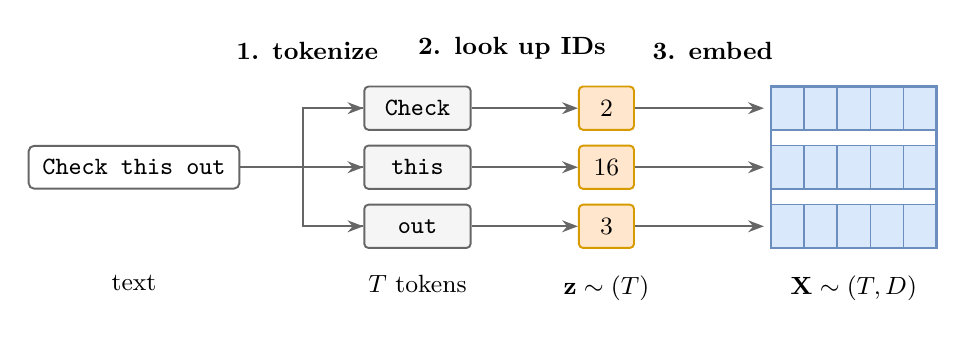
\begin{tikzpicture}[x=1cm,y=1cm,
        tok/.style={draw=drawgray,fill=drawgray_l,rounded corners=1.5pt,line width=0.7pt,
            minimum width=1.35cm,minimum height=0.55cm,inner sep=2pt,font=\small\ttfamily},
        tid/.style={draw=draworange,fill=draworange_l,rounded corners=1.5pt,line width=0.7pt,
            minimum width=0.7cm,minimum height=0.55cm,inner sep=0pt,font=\small},
        ecell/.style={draw=drawblue,fill=drawblue_l,line width=0.5pt,minimum width=0.42cm,
            minimum height=0.55cm,inner sep=0pt},
        edge/.style={-{Stealth[length=2mm]},line width=0.8pt,draw=drawgray},
        steplab/.style={font=\small\bfseries,anchor=south,align=center},
        under/.style={font=\small,anchor=north}]
    \node[draw=drawgray,rounded corners=2pt,line width=0.7pt,inner sep=5pt,
        font=\small\ttfamily] (text) at (0,0) {Check this out};
    \foreach \w/\id [count=\t from 0] in {Check/2,this/16,out/3}{
        \pgfmathsetmacro{\y}{0.75-0.75*\t}
        \node[tok] (w\t) at (3.6,\y) {\w};
        \node[tid] (z\t) at (6.0,\y) {$\id$};
        \foreach \d in {0,...,4}{
            \node[ecell] at (8.3+0.42*\d,\y) {};
        }
        \draw[edge] (w\t.east) -- (z\t.west);
        \draw[edge] (z\t.east) -- (8.0,\y);
        \draw[drawgray,line width=0.7pt] (text.east) -- (2.15,0) |- (w\t.west);
    }
    \draw[edge] (2.15,0.75) -- (w0.west);
    \draw[edge] (2.15,0) -- (w1.west);
    \draw[edge] (2.15,-0.75) -- (w2.west);
    \draw[drawblue,line width=1pt] (8.09,1.025) rectangle (10.19,-1.025);
    \node[steplab] at (2.2,1.25) {1. tokenize};
    \node[steplab] at (4.8,1.25) {2. look up IDs};
    \node[steplab] at (7.35,1.25) {3. embed};
    \node[under] at (0,-1.25) {text};
    \node[under] at (3.6,-1.25) {$T$ tokens};
    \node[under] at (6.0,-1.25) {$\vc{z}\sim(T)$};
    \node[under] at (9.14,-1.25) {$\vc{X}\sim(T,D)$};
\end{tikzpicture}
\endgroup

    \end{center}

    \vspace{0.5em}
    {\raggedright
        By the end of this procedure we have a matrix $\vc{X}\sim(T,D)$ of $T$
        tokens, each represented by $D$ features\NNDSorNN{}{ (we write $\vc{X}\sim(T,D)$ for a matrix with $T$ rows and $D$ columns)}.\par}

\end{whiteframe}

\begin{whiteframe}{Step 1: choosing the tokens}
    \setlength{\parskip}{4pt}

    We first choose how to split (\myalert{tokenize}) the text, e.g., by
    character, by byte, by \myalert{subword} or by word:

    \begin{center}
        % Editable tokenization comparison on one sentence: characters, subwords and
% words, with the resulting sequence length. Subwords are the actual output of
% the GPT-4 tokenizer (tiktoken, cl100k_base). Written by Claude (2026-10-30),
% replacing the old tokenization figure.
\begingroup
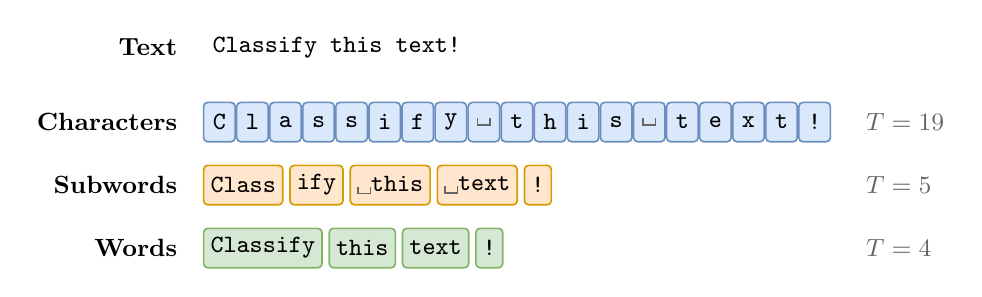
\begin{tikzpicture}[x=1cm,y=1cm,
        tk/.style={draw=#1,fill=#1_l,rounded corners=1.5pt,line width=0.6pt,
            minimum height=0.5cm,inner sep=2.5pt,font=\small\ttfamily,anchor=west},
        rowlabel/.style={font=\small\bfseries,anchor=east},
        len/.style={font=\small,anchor=west,text=drawgray}]
    % Visible space drawn with rules: the monospace font has no U+2423 glyph.
    \def\sp{{\color{drawgray}\rule[-0.3ex]{0.5pt}{0.7ex}\rule[-0.3ex]{0.42em}{0.5pt}\rule[-0.3ex]{0.5pt}{0.7ex}}}
    \node[font=\small\ttfamily,anchor=west] at (0,0.95) {Classify this text!};
    \node[rowlabel] at (-0.2,0.95) {Text};
    % Characters (spaces are tokens too).
    \node[rowlabel] at (-0.2,0) {Characters};
    \foreach \ch [count=\n from 0] in {C,l,a,s,s,i,f,y,\sp,t,h,i,s,\sp,t,e,x,t,!}{
        \node[tk=drawblue,minimum width=0.4cm,inner sep=0pt] at (0.42*\n,0) {\ch};
    }
    \node[len] at (8.3,0) {$T=19$};
    % Subwords.
    \node[rowlabel] at (-0.2,-0.8) {Subwords};
    \node[tk=draworange] (s0) at (0,-0.8) {Class};
    \node[tk=draworange] (s1) at ([xshift=2pt]s0.east) {ify};
    \node[tk=draworange] (s2) at ([xshift=2pt]s1.east) {\sp this};
    \node[tk=draworange] (s3) at ([xshift=2pt]s2.east) {\sp text};
    \node[tk=draworange] (s4) at ([xshift=2pt]s3.east) {!};
    \node[len] at (8.3,-0.8) {$T=5$};
    % Words.
    \node[rowlabel] at (-0.2,-1.6) {Words};
    \node[tk=drawgreen] (v0) at (0,-1.6) {Classify};
    \node[tk=drawgreen] (v1) at ([xshift=2pt]v0.east) {this};
    \node[tk=drawgreen] (v2) at ([xshift=2pt]v1.east) {text};
    \node[tk=drawgreen] (v3) at ([xshift=2pt]v2.east) {!};
    \node[len] at (8.3,-1.6) {$T=4$};
\end{tikzpicture}
\endgroup

    \end{center}

    Larger \myalert{tokens} give shorter sequences, but we need many more of
    them to cover all possible texts. Byte tokenization works like character
    tokenization on the $256$ byte values of UTF-8 text.

    \SlideSource{Subwords from the GPT-4 tokenizer (\texttt{cl100k\_base}), via
        \href{https://github.com/openai/tiktoken}{tiktoken}.}

\end{whiteframe}

\begin{frame}{Step 1: building the vocabulary}
    \setlength{\parskip}{4pt}

    The set of tokens we can handle is the \myalert{vocabulary} or
    \myalert{dictionary}. Its size $V$ depends on the type of token:

    \medskip
    \begin{columns}[T,onlytextwidth]
        \begin{column}{0.32\textwidth}
            \begin{tcolorbox}[nndsblue,courseheight={text-vocab}{}]
                \textbf{Characters or bytes}\\
                A small fixed set, e.g., the $256$ byte values.
            \end{tcolorbox}
        \end{column}
        \begin{column}{0.32\textwidth}
            \begin{tcolorbox}[nndsred,courseheight={text-vocab}{}]
                \textbf{Words}\\
                The $V$ most frequent words of a training corpus, plus a
                special \textit{unknown} token.
            \end{tcolorbox}
        \end{column}
        \begin{column}{0.32\textwidth}
            \begin{tcolorbox}[nndsgreen,courseheight={text-vocab}{}]
                \textbf{Subwords}\\
                Reusable pieces learned from a corpus, e.g., with
                \myalert{byte pair encoding} (BPE).
            \end{tcolorbox}
        \end{column}
    \end{columns}

    \medskip
    Larger tokens need a larger vocabulary: a few hundred characters, but
    tens of thousands of words or subwords.

\end{frame}

\begin{frame}{Subword embeddings}
    \setlength{\parskip}{3pt}
    \setlength{\abovedisplayskip}{6pt}
    \setlength{\belowdisplayskip}{6pt}

    Word-level vocabularies can miss unseen words. Character tokenization
    produces longer sequences. With \myalert{subword tokenization}, we reuse
    pieces across words, for example (illustrative):
    \[
        \begin{array}{rcl}
            \texttt{playing} & \longmapsto & (\texttt{play},\texttt{ing}) \\
            \texttt{played}  & \longmapsto & (\texttt{play},\texttt{ed})
        \end{array}
    \]

    Each piece has an ID and a row in $\vc{E}\sim(V,D)$.
    Both words share the embedding for \texttt{play}.

    Unseen words can split into known pieces, and frequent words can stay whole.
    Learned pieces need not match linguistic word parts.

    \SlideSource{Sennrich, Haddow and Birch (2016),
        \href{https://aclanthology.org/P16-1162/}{\textit{Neural Machine Translation of Rare Words with Subword Units}}, ACL.}

\end{frame}

\begin{frame}{Byte pair encoding}
    \setlength{\parskip}{3pt}
    \setlength{\abovedisplayskip}{5pt}
    \setlength{\belowdisplayskip}{5pt}

    We can learn the vocabulary with \myalert{byte pair encoding} (BPE):
    \begin{enumerate}
        \item Start the vocabulary with the single characters.
        \item Merge the most frequent adjacent pair into a new token, \myalert{added to the vocabulary}.
        \item Repeat until the vocabulary reaches the chosen size $V$.
    \end{enumerate}

    Toy corpus: \texttt{hug} $\times5$, \texttt{hugs} $\times3$,
    \texttt{pug} $\times2$. We count pairs within words:
    \[
        \begin{array}{rcll}
            (\texttt{u},\texttt{g})  & \longmapsto & \texttt{ug}  & \quad 10\text{ occurrences} \\
            (\texttt{h},\texttt{ug}) & \longmapsto & \texttt{hug} & \quad 8\text{ occurrences}
        \end{array}
    \]
    The vocabulary grows from $\{\texttt{g},\texttt{h},\texttt{p},\texttt{s},\texttt{u}\}$
    to $\{\ldots,\texttt{ug}\}$ and then $\{\ldots,\texttt{ug},\texttt{hug}\}$.

    On new text, we apply the fixed merge rules in their learned order.
    \myalert{Byte-level BPE} starts from $256$ byte values, so it can represent
    any UTF-8 text.

    \SlideSource{\href{https://huggingface.co/learn/llm-course/en/chapter6/5}{Hugging Face: Byte-Pair Encoding tokenization}.}

\end{frame}

% Figure: shared/assets/images/text/vocabulary.tex (Claude, 2026-10-30).
\begin{whiteframe}{Step 2: from tokens to IDs}
    \setlength{\parskip}{4pt}

    Each token in the text is converted into a discrete ID
    $z_t\in\{0,\ldots,V-1\}$, its position in the vocabulary, giving us an
    integer sequence $\vc{z}\sim(T)$:

    \begin{center}
        % Editable word-level vocabulary: a table of IDs and tokens, and the lookup
% of two texts, one with a typo that falls back to the unknown token. IDs
% match the embedding-lookup slide (Check = 2, this = 16, out = 3).
% Written by Claude (2026-10-30).
\begingroup
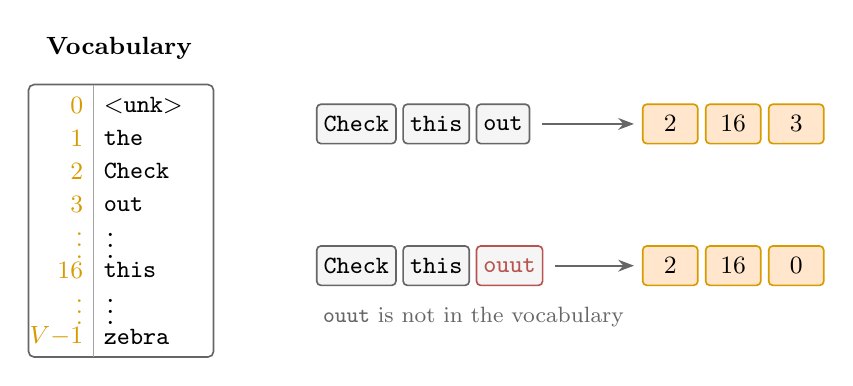
\begin{tikzpicture}[x=1cm,y=1cm,
        vrow/.style={minimum height=0.42cm,inner sep=0pt,font=\small},
        tok/.style={draw=drawgray,fill=drawgray_l,rounded corners=1.5pt,line width=0.6pt,
            minimum height=0.5cm,inner sep=2.5pt,font=\small\ttfamily},
        tid/.style={draw=draworange,fill=draworange_l,rounded corners=1.5pt,line width=0.6pt,
            minimum width=0.7cm,minimum height=0.5cm,inner sep=0pt,font=\small},
        edge/.style={-{Stealth[length=2mm]},line width=0.8pt,draw=drawgray},
        head/.style={font=\small\bfseries,anchor=south}]
    % Vocabulary table.
    \node[head] at (0.9,1.45) {Vocabulary};
    \foreach \id/\tk [count=\n from 0] in {
            0/{\textless unk\textgreater},1/{the},2/{Check},3/{out},
            \vdots/{\vdots},16/{this},\vdots/{\vdots},V{-}1/{zebra}}{
        \pgfmathsetmacro{\y}{1.2-0.42*\n}
        \node[vrow,anchor=east,text=draworange] at (0.45,\y-0.21) {$\id$};
        \node[vrow,anchor=west,font=\small\ttfamily] at (0.7,\y-0.21) {\tk};
    }
    \draw[drawgray,line width=0.6pt,rounded corners=2pt] (-0.25,1.25) rectangle (2.1,-2.21);
    \draw[drawgray!60,line width=0.4pt] (0.58,1.25) -- (0.58,-2.21);

    % Two lookups.
    \foreach \row/\yy in {0/0.75,1/-1.05}{
        \ifcase\row
            \node[tok,anchor=west] (a\row) at (3.4,\yy) {Check};
            \node[tok,anchor=west] (b\row) at ([xshift=2pt]a\row.east) {this};
            \node[tok,anchor=west] (c\row) at ([xshift=2pt]b\row.east) {out};
        \or
            \node[tok,anchor=west] (a\row) at (3.4,\yy) {Check};
            \node[tok,anchor=west] (b\row) at ([xshift=2pt]a\row.east) {this};
            \node[tok,anchor=west,draw=drawred,text=drawred] (c\row) at ([xshift=2pt]b\row.east) {ouut};
        \fi
    }
    \foreach \row/\yy/\ids in {0/0.75/{2,16,3},1/-1.05/{2,16,0}}{
        \foreach \i [count=\n from 0] in \ids{
            \node[tid] (i\row\n) at (7.9+0.8*\n,\yy) {$\i$};
        }
        \draw[edge] ([xshift=0.15cm]c\row.east) -- ([xshift=-0.1cm]i\row0.west);
    }
    \node[font=\footnotesize,text=drawgray,anchor=north] at (5.4,-1.45)
        {\texttt{ouut} is not in the vocabulary};
\end{tikzpicture}
\endgroup

    \end{center}

    A word outside the vocabulary, such as a typo, becomes the unknown token.

\end{whiteframe}

\begin{frame}{Step 3: dense embeddings}
    \setlength{\parskip}{4pt}
    \setlength{\abovedisplayskip}{7pt}
    \setlength{\belowdisplayskip}{7pt}

    For embedding we learn an \myalert{embedding matrix} $\vc{E}\sim(V,D)$, with one row for each of the $V$ tokens in the vocabulary. Embedding element $z_t$ of the sequence is just a row lookup:
    \[
        \idx{\vc{X}}{t,:}=\idx{\vc{E}}{z_t,:}
    \]

    We initialize the embeddings randomly and train them with the network, or take them from some pre-trained model or algorithm.
    For example, GloVe and Word2Vec were two classic algorithms for this purpose.

    Pre-trained embeddings also inherit the biases of their training text:
    for example, word analogies can reproduce gender stereotypes about
    professions.

    \SlideSource{Bolukbasi et al. (2016), \href{https://arxiv.org/abs/1607.06520}{\textit{Man is to Computer Programmer as Woman is to Homemaker? Debiasing Word Embeddings}}, NeurIPS.}

\end{frame}

% Figure: shared/assets/images/text/embedding_lookup.tex (Claude, 2026-10-30).
\begin{whiteframe}{Visualizing the embedding procedure}

    \vspace{0.5em}
    \begin{center}
        % Editable embedding lookup: the IDs of "Check this out" select rows of
% E ~ (V,D), which become the rows of X ~ (T,D), the input of a 1D CNN (NNDS) or a transformer (NN).
% Written by Claude (2026-10-30), replacing the old embedding figure.
\begingroup
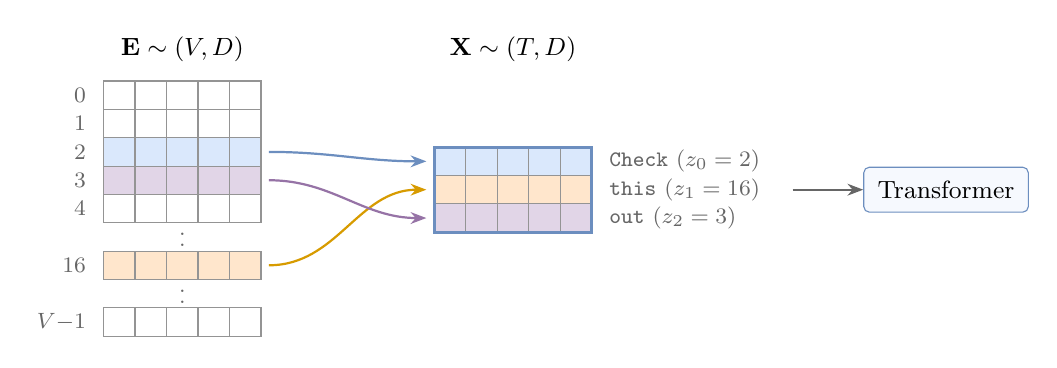
\begin{tikzpicture}[x=1cm,y=1cm,
        ecell/.style={draw=drawgray!70,line width=0.4pt,minimum width=0.4cm,
            minimum height=0.36cm,inner sep=0pt},
        tid/.style={draw=draworange,fill=draworange_l,rounded corners=1.5pt,line width=0.6pt,
            minimum width=0.7cm,minimum height=0.5cm,inner sep=0pt,font=\small},
        edge/.style={-{Stealth[length=2mm]},line width=0.8pt,draw=drawgray},
        lab/.style={font=\small},
        note/.style={font=\footnotesize,text=drawgray}]
    % Embedding matrix: displayed rows, with the ID of each row on the left.
    \foreach \id/\fill [count=\n from 0] in {
            0/white,1/white,2/drawblue_l,3/drawviolet_l,4/white,
            dots/white,16/draworange_l,dots/white,V{-}1/white}{
        \pgfmathsetmacro{\y}{1.6-0.36*\n}
        \def\tmp{dots}
        \ifx\id\tmp
            \node[note] at (1.0,\y) {$\vdots$};
        \else
            \foreach \d in {0,...,4}{
                \node[ecell,fill=\fill] at (0.2+0.4*\d,\y) {};
            }
            \node[note,anchor=east] at (-0.1,\y) {$\id$};
        \fi
    }
    \node[lab,anchor=south] at (1.0,1.9) {$\vc{E}\sim(V,D)$};

    % X: one row per token.
    \begin{scope}[shift={(4.2,0)}]
        \foreach \fill/\w/\id [count=\t from 0] in {drawblue_l/Check/2,draworange_l/this/16,drawviolet_l/out/3}{
            \foreach \d in {0,...,4}{
                \node[ecell,fill=\fill] at (0.2+0.4*\d,0.76-0.36*\t) {};
            }
            \node[note,anchor=west] at (2.1,0.76-0.36*\t) {\texttt{\w} ($z_{\t}=\id$)};
        }
        \node[lab,anchor=south] at (1.0,1.9) {$\vc{X}\sim(T,D)$};
    \end{scope}
    % Row copies.
    \draw[edge,draw=drawblue] (2.1,0.88) to[out=0,in=180] (4.1,0.76);
    \draw[edge,draw=draworange] (2.1,-0.56) to[out=0,in=180] (4.1,0.40);
    \draw[edge,draw=drawviolet] (2.1,0.52) to[out=0,in=180] (4.1,0.04);
    % Next layer.
    \node[lab,draw=drawblue,fill=drawblue_l!25!white,rounded corners=2pt,
        inner sep=5pt] (cnn) at (10.7,0.4) {\NNDSorNN{1D CNN}{Transformer}};
    \draw[drawblue,line width=1pt] (4.2,0.94) rectangle (6.2,-0.14);
    \draw[edge] (8.75,0.4) -- (cnn.west);
\end{tikzpicture}
\endgroup

    \end{center}

    \vspace{0.6em}
    For $\vc{z}=(2,16,3)$, each ID selects one row of $\vc{E}$. With custom embeddings, we train
    $\vc{E}$ together with the rest of the network\NNDSorNN{, e.g., a 1D CNN for text
    classification}{}.

\end{whiteframe}

\begin{frame}{Sequence padding}
    \setlength{\parskip}{4pt}
    \setlength{\abovedisplayskip}{7pt}
    \setlength{\belowdisplayskip}{7pt}

    Two texts may have different lengths. Their embedded matrices
    $\vc{X}_1\sim(T_1,D)$ and $\vc{X}_2\sim(T_2,D)$ share the same feature dimension $D$.

    For $T_1>T_2$, we can build a padded mini-batch:
    \[
        X=\operatorname{stack}\!\left(
        \vc{X}_1,\begin{bmatrix}\vc{X}_2\\\vc{0}\end{bmatrix}
        \right),
        \qquad X\sim(2,T_1,D).
    \]

    We pad to the maximum sequence length in the mini-batch.
    The added zero rows are placeholders.

    We keep a \myalert{validity mask} of real positions, so padded positions
    do not contribute to pooling or to the loss.

\end{frame}



% Transformer lecture shared by NN and NNDS. Moved from the NNDS deck
% Lecture_transformers.tex by Claude (2026-11-16) for the NN transformer deck.
% \NNDSorNN{NNDS text}{NN text} holds the few course-specific sentences, and
% \ifNNcourse ... \else ... \fi the frames that differ. NN students arrive from
% recurrent models, NNDS students from the CNN lecture (1D and causal
% convolutions), so the NN frames motivate attention from recurrence.

% Token rows for the "Three ways to weight a neighbor" figure.
\def\tokdx{0.85}
\def\tokyo{2.3}
\newcommand{\panelrows}[2]{%
    \foreach \i in {0,...,4} {
            \node[tok] (o#1\i) at ({#2+\i*\tokdx},\tokyo) {};
            \node[tok] (i#1\i) at ({#2+\i*\tokdx},0) {};
        }
    \node[outtok] at (o#12) {};
    \node[gtok] at (i#11) {};
    \node[btok] at (i#14) {};
    \node[vlab, above=1pt] at (o#12.north) {$\vc{h}_t$};
    \node[vlab, below=1pt, drawgreen!70!black] at (i#11.south) {$\vc{x}_{t-1}$};
    \node[vlab, below=1pt, drawblue!80!black] at (i#14.south) {$\vc{x}_{t+2}$};
}



\section{Designing the transformer}
\subsection{\NNDSorNN{From convolutions to attention}{From recurrence to attention}}

\begin{frame}{Transformers}
    \setlength{\parskip}{4pt}

    The \myalert{transformer} was proposed in 2017 for machine translation. \NNDSorNN{Like the convolutional models of the
        last lecture,}{Like the recurrent models of the
        previous lectures,} the backbone maps a sequence of embeddings $\vc{X} \sim(T,D)$ to another sequence followed by a task-specific head, e.g.:

    \vspace{0.2em}
    \begin{columns}[T,onlytextwidth]
        \begin{column}{0.48\textwidth}
            \begin{tcolorbox}[nndsblue,courseheight={families}{}]
                \textbf{Sequence classification}\par
                Each output can depend on the whole sequence: we call it an
                \myalert{encoder} transformer (e.g. BERT, ViT).
            \end{tcolorbox}
        \end{column}
        \begin{column}{0.48\textwidth}
            \begin{tcolorbox}[nndsred,courseheight={families}{}]
                \textbf{Next-token prediction}\par
                The model must be causal, \NNDSorNN{as with causal convolutions}{as in a recurrent model}: we call it a \myalert{decoder} transformer (e.g. GPT).
            \end{tcolorbox}
        \end{column}
    \end{columns}

    \vspace{0.6em}
    As we will see, the original 2017 paper combined both.

    \SlideSource{Vaswani et al. (2017), \href{https://arxiv.org/abs/1706.03762}{\textit{Attention is all you need}}, NeurIPS.}

\end{frame}

\ifNNcourse
    \begin{frame}{Beyond recurrence}
        \setlength{\parskip}{6pt}

        A recurrent model reads the tokens one at a time and summarizes the past
        in a state of fixed size, $\vc{h}_t=f(\vc{h}_{t-1},\vc{x}_t)$. This has
        two drawbacks:
        \begin{itemize}
            \item \textbf{Long-range dependencies:} information from token $t-k$
                  reaches token $t$ through $k$ state updates, and the
                  gradients through many updates tend to vanish or explode.
            \item \textbf{Sequential computation:} $\vc{h}_t$ needs
                  $\vc{h}_{t-1}$, so even with teacher forcing we cannot process
                  the positions of a sequence in parallel.
        \end{itemize}
        Compare:
        \begin{itemize}
            \item \textit{the {\color{darkcerulean}\textbf{cat}} is on the {\color{darkgreen}\textbf{table}}};
            \item \textit{the {\color{darkcerulean}\textbf{cat}}, which belonged to my mother, is on the {\color{darkgreen}\textbf{table}}}.
        \end{itemize}
        The relation between the two words is the same, but their distance is not.
        We want a layer where every output reads every token directly, and all
        outputs are computed in parallel.

    \end{frame}
\else
    \begin{frame}{Beyond locality}
        \setlength{\parskip}{6pt}

        A convolution assumes \myalert{locality}: each output mixes a fixed window
        of neighbors. In text, audio or graphs, dependencies can instead be
        \myalert{long-range}, \myalert{sparse} and \myalert{dynamic}.

        Compare:
        \begin{itemize}
            \item \textit{the {\color{darkcerulean}\textbf{cat}} is on the {\color{darkgreen}\textbf{table}}};
            \item \textit{the {\color{darkcerulean}\textbf{cat}}, which belonged to my mother, is on the {\color{darkgreen}\textbf{table}}}.
        \end{itemize}
        The relation between the two words is the same, but their distance is not.

        Stacking layers (or dilating them) grows the receptive field. However, the
        weight given to a neighbor still depends only on its \textit{offset}, never on
        what the two tokens contain.

    \end{frame}
\fi

\begin{frame}{Convolutions as a sum over offsets}
    \setlength{\parskip}{6pt}

    Take a sequence $\vc{X}\sim(T,D)$ with rows $\vc{x}_t=\idx{\vc{X}}{t,:}$. Because
    transformers come from NLP, we call each row a \myalert{token} and $D$ the
    \myalert{embedding dimension}.

    \NNDSorNN{Ignoring padding and the activation, a 1D convolution with kernel size
        $s=2k+1$ is:}{A 1D convolution, the sequence version of the image
        convolutions of the CNN lecture, processes all tokens in parallel. Ignoring
        padding and the activation, with kernel size $s=2k+1$:}
    \[
        \vc{h}_t=\sum_{j=-k}^{k}\eqnmarkbox[drawblue]{wconv}{\idx{\vc{W}}{j+k,:,:}}\,\vc{x}_{t+j}\,,
        \qquad \vc{W}\sim(s,D,D).
    \]
    \annotate[yshift=-0.8em]{below,right}{wconv}{one matrix per offset}
    \vspace{0.6em}

    \NNDSorNN{This is the layer of the CNN lecture, with the kernel reshaped into one
        $D\times D$ matrix for each offset $j$, stored at position $j+k$. Its parameters grow linearly with
        $s$. We want to remove the locality assumption while keeping the number of
        parameters independent of the length $T$.}{The kernel has one $D\times D$
        matrix for each offset $j$, so its parameters grow linearly with $s$. Each
        output sees only a window of $s$ tokens (\myalert{locality}), and the
        weight of a neighbor depends only on its offset, never on what the two
        tokens contain. We want to remove both limits while keeping the number of
        parameters independent of the length $T$.}

\end{frame}

\begin{frame}{Continuous convolutions}
    \setlength{\parskip}{6pt}

    Instead of storing one matrix per offset, we \textit{compute} it with a small
    trainable network $g:\mathbb{Z}\rightarrow\mathbb{R}^{D\times D}$ that takes
    the offset as input:
    \[
        \vc{h}_t=\sum_{t'=0}^{T-1}\eqnmarkbox[drawblue]{wcont}{g(t'-t)}\,\vc{x}_{t'}\,.
    \]
    \annotate[yshift=-0.8em]{below,right}{wcont}{weight computed from the offset}
    \vspace{0.6em}

    The kernel now covers the whole sequence with a fixed number of
    parameters. These \myalert{continuous convolutions} also handle inputs of
    variable size and resolution.

    \SlideSource{Romero et al. (2022), \href{https://arxiv.org/abs/2206.03398}{\textit{Towards a General Purpose CNN for Long Range Dependencies in $N$D}}, arXiv.}

\end{frame}

\begin{frame}{Non-local networks}
    \setlength{\parskip}{6pt}

    A continuous convolution handles long-range dependencies, but they are
    still \textit{regular}: the weight depends only on the offset $t'-t$. We
    can let it depend on the \textit{values} of the tokens instead:
    \[
        \vc{h}_t=\sum_{t'=0}^{T-1}\eqnmarkbox[drawblue]{wnl}{\alpha(\vc{x}_t,\vc{x}_{t'})}\,\vc{x}_{t'}\,.
    \]
    \annotate[yshift=-0.8em]{below,right}{wnl}{weight computed from the two tokens}
    \vspace{0.6em}

    This is a \myalert{non-local neural network}. With a suitable choice of
    the weighting function $\alpha$, we will obtain the attention layer.$^1$

    \vfill
    {\footnotesize\color{black!60} $^1$ We could also combine the two ideas, with a
        weight $\alpha(\vc{x}_t,\vc{x}_{t'},t'-t)$ that depends on both the tokens and
        their offset. We will return to this with \textit{relative positional
            embeddings}.\par}

    \SlideSource{Wang et al. (2018), \href{https://arxiv.org/abs/1711.07971}{\textit{Non-local Neural Networks}}, CVPR.}

\end{frame}

\begin{frame}{Three ways to weight a neighbor}
    % Redrawn in TikZ by Claude (2026-10-27); the 2024 draw.io version is kept in
    % shared/assets/images/transformers/book/convolution_types.drawio.
    \centering
    \vspace{0.4em}
    \begin{tikzpicture}[
            tok/.style={circle, draw=drawgray!50, fill=white, line width=0.6pt, minimum size=0.62cm, inner sep=0pt},
            outtok/.style={tok, draw=drawred, fill=drawred!22},
            gtok/.style={tok, draw=drawgreen, fill=drawgreen_l},
            btok/.style={tok, draw=drawblue, fill=drawblue_l},
            edge/.style={drawgray!40, line width=0.5pt},
            gedge/.style={drawgreen!80!black, line width=1pt},
            bedge/.style={drawblue!80!black, line width=1pt},
            wlab/.style={font=\footnotesize, fill=white, inner sep=1.5pt},
            vlab/.style={font=\footnotesize},
            ptitle/.style={font=\small},
        ]
        % (a) Convolution with s = 3: weights only inside the window.
        \panelrows{a}{0}
        \draw[edge] (oa2.south) -- (ia2.north);
        \draw[edge] (oa2.south) -- (ia3.north);
        \draw[gedge] (oa2.south) -- node[wlab, pos=0.5, left=6pt] {$\idx{\vc{W}}{0,:,:}$} (ia1.north);
        \draw[bedge, dashed, drawblue!60] (oa2.south) -- node[wlab, pos=0.5, right=6pt, text=drawgray] {no weight} (ia4.north);
        \node[ptitle] at ({2*\tokdx},-1.1) {(a) Convolution, $s=3$};

        % (b) Continuous convolution: weights computed from the offset.
        \panelrows{b}{4.7}
        \foreach \i in {0,2,3} {\draw[edge] (ob2.south) -- (ib\i.north);}
        \draw[gedge] (ob2.south) -- node[wlab, pos=0.5, left=6pt] {$g(-1)$} (ib1.north);
        \draw[bedge] (ob2.south) -- node[wlab, pos=0.5, right=6pt] {$g(+2)$} (ib4.north);
        \node[ptitle] at ({4.7+2*\tokdx},-1.1) {(b) Continuous convolution};

        % (c) Non-local network: weights computed from the two tokens.
        \panelrows{c}{9.35}
        \foreach \i in {0,2,3} {\draw[edge] (oc2.south) -- (ic\i.north);}
        \draw[gedge] (oc2.south) -- node[wlab, pos=0.5, left=6pt] {$\alpha(\vc{x}_t,\vc{x}_{t-1})$} (ic1.north);
        \draw[bedge] (oc2.south) -- node[wlab, pos=0.5, right=6pt] {$\alpha(\vc{x}_t,\vc{x}_{t+2})$} (ic4.north);
        \node[ptitle] at ({9.35+2*\tokdx},-1.1) {(c) Non-local network};
    \end{tikzpicture}

    \vspace{0.8em}
    {\small Each edge weights an input token for the output $\vc{h}_t$: (a) one
        matrix per offset, inside the kernel only; (b) computed from the offset; (c)
        computed from the two tokens.\par}

\end{frame}

\subsection{Self-attention}

\begin{frame}{Choosing the weighting function}
    \setlength{\parskip}{6pt}

    We now design $\alpha$. Two simplifications make it cheap and stable:
    \begin{itemize}
        \item \textbf{Scalar weights:} $\alpha$ returns a number, not a
              $D\times D$ matrix, so $\vc{h}_t$ is a weighted average of the
              tokens.
        \item \textbf{Normalized weights:} for each $t$, the weights are
              positive and sum to one over $t'$. Each token has a
              \textit{budget} of attention: raising one weight lowers the
              others.
    \end{itemize}

    Both follow from a \myalert{scoring function} $s$ and a softmax over $t'$:
    \[
        \alpha(\vc{x}_t,\vc{x}_{t'})
        =\frac{\exp\left(s(\vc{x}_t,\vc{x}_{t'})\right)}
        {\sum_{r=0}^{T-1}\exp\left(s(\vc{x}_t,\vc{x}_{r})\right)} \,.
    \]
    We call $\alpha(\vc{x}_t,\vc{x}_{t'})$ the \myalert{attention weight}
    of token $t$ on token $t'$.

\end{frame}

\begin{frame}{Dot-product attention}
    \setlength{\parskip}{6pt}

    The most common score is the scaled dot product, $s(\vc{x}_t,\vc{x}_{t'})
        =\vc{x}_t^{\top}\vc{x}_{t'}/\sqrt{D}$. All pairs come from one matrix
    product, which is fast on a GPU. Putting everything together:
    \[
        \vc{h}_t=\sum_{t'=0}^{T-1}
        \eqnmarkbox[drawblue]{sm}{\operatorname{softmax}_{t'}}
        \left(\frac{\vc{x}_t^{\top}\vc{x}_{t'}}{\sqrt{D}}\right)\vc{x}_{t'} \,.
    \]
    \annotate[yshift=-0.8em]{below,right}{sm}{normalized over $t'$}
    \vspace{0.6em}

    This is already an attention layer, without any parameters.$^1$

    \vfill
    {\footnotesize\color{black!60} $^1$ Why $\sqrt{D}$? If the elements of
        $\vc{x}_t$ and $\vc{x}_{t'}$ ($t'\neq t$) are independent with mean $0$
        and variance $\sigma^2$, then $\operatorname{Var}(\vc{x}_t^{\top}\vc{x}_{t'})=D\sigma^4$
        (check!). Without the scaling, the scores grow with $D$ and a single large
        score saturates the softmax.\par}

\end{frame}

\begin{frame}{Queries, keys and values}
    \setlength{\parskip}{6pt}

    So far the same vector plays three roles. We give each role its own
    trainable projection:
    \[
        \qc{\vc{q}_t=\vc{W}_q^{\top}\vc{x}_t}, \qquad
        \kc{\vc{k}_t=\vc{W}_k^{\top}\vc{x}_t}, \qquad
        \vcl{\vc{v}_t=\vc{W}_v^{\top}\vc{x}_t},
    \]
    with $\vc{W}_q,\vc{W}_k\sim(D,D_k)$ and $\vc{W}_v\sim(D,D_v)$. The
    complete \myalert{self-attention} (SA) layer is:
    \[
        \vc{h}_t=\sum_{t'=0}^{T-1}\operatorname{softmax}_{t'}
        \left(\frac{\qc{\vc{q}_t^{\top}}\kc{\vc{k}_{t'}}}{\sqrt{D_k}}\right)\vcl{\vc{v}_{t'}} \,.
    \]
    The scores are no longer necessarily symmetric. Value projection by $\vc{W}_v$ allows for feature mixing.

\end{frame}

\begin{frame}{Self-attention in matrix form}
    \setlength{\parskip}{4pt}

    Stacking the tokens in $\vc{X}\sim(T,D)$, the projections are three
    matrix products:
    \[
        \qc{\shape{\vc{Q}}{(T,D_k)}=\vc{X}\vc{W}_q}, \qquad
        \kc{\shape{\vc{K}}{(T,D_k)}=\vc{X}\vc{W}_k}, \qquad
        \vcl{\shape{\vc{V}}{(T,D_v)}=\vc{X}\vc{W}_v}.
    \]
    The whole layer is then:
    \[
        \shape{\vc{H}}{(T,D_v)}
        =\eqnmarkbox[drawblue]{amat}{\operatorname{softmax}\left(\frac{\qc{\vc{Q}}\kc{\vc{K}}^{\top}}{\sqrt{D_k}}\right)}
        \vcl{\vc{V}} \,.
    \]
    \annotate[yshift=-0.8em]{below,right}{amat}{attention matrix $\vc{A}\sim(T,T)$, softmax on each row}
    \vspace{0.6em}

    Row $t$ of $\vc{A}$ holds the attention weights of token $t$. In a batch
    $\vc{X}\sim(B,T,D)$, tokens attend only within their own sequence. The need to compute
    $T^2$ entries for $\vc{A}$ is a potential bottleneck for long sequences (more on this later on).

\end{frame}

\begin{frame}{Visualizing self-attention}
    \centering
    \vspace{1em}
    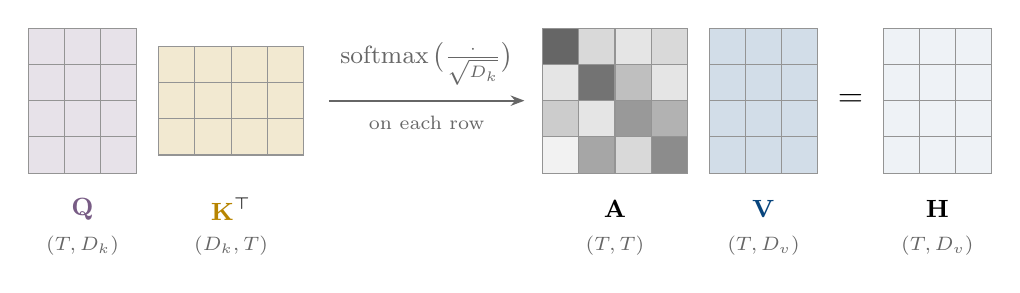
\begin{tikzpicture}[x=0.46cm, y=0.46cm,
            cell/.style={draw=drawgray!70, line width=0.4pt},
            mlab/.style={font=\small},
            slab/.style={font=\scriptsize, text=black!60},
        ]
        % Q (T x D_k)
        \foreach \r in {0,...,3} \foreach \c in {0,...,2}
        \draw[cell, fill=qcolor!18] (\c,-\r) rectangle ++(1,-1);
        \node[mlab] at (1.5,-5) {$\qc{\vc{Q}}$};
        \node[slab] at (1.5,-6) {$(T,D_k)$};
        % K^T (D_k x T)
        \foreach \r in {0,...,2} \foreach \c in {0,...,3}
        \draw[cell, fill=kcolor!18] ({3.6+\c},{-0.5-\r}) rectangle ++(1,-1);
        \node[mlab] at (5.6,-5) {$\kc{\vc{K}}^{\top}$};
        \node[slab] at (5.6,-6) {$(D_k,T)$};
        % softmax arrow
        \draw[-{Stealth[length=5pt]}, drawgray, line width=0.6pt] (8.3,-2) -- (13.7,-2)
        node[midway, above=2pt, font=\small] {$\operatorname{softmax}\big(\tfrac{\cdot}{\sqrt{D_k}}\big)$}
        node[midway, below=2pt, slab] {on each row};
        % A (T x T), row-normalized weights
        \def\arow{{60,15,10,15},{10,55,25,10},{20,10,40,30},{5,35,15,45}}
        \foreach \row [count=\r from 0] in \arow {
            \foreach \v [count=\c from 0] in \row {
                \draw[cell, fill=black!\v] ({14.2+\c},-\r) rectangle ++(1,-1);
            }
        }
        \node[mlab] at (16.2,-5) {$\vc{A}$};
        \node[slab] at (16.2,-6) {$(T,T)$};
        % V (T x D_v)
        \foreach \r in {0,...,3} \foreach \c in {0,...,2}
        \draw[cell, fill=vcolor!18] ({18.8+\c},-\r) rectangle ++(1,-1);
        \node[mlab] at (20.3,-5) {$\vcl{\vc{V}}$};
        \node[slab] at (20.3,-6) {$(T,D_v)$};
        \node[font=\large] at (22.7,-2) {$=$};
        % H (T x D_v)
        \foreach \r in {0,...,3} \foreach \c in {0,...,2}
        \draw[cell, fill=vcolor!7] ({23.6+\c},-\r) rectangle ++(1,-1);
        \node[mlab] at (25.1,-5) {$\vc{H}$};
        \node[slab] at (25.1,-6) {$(T,D_v)$};
    \end{tikzpicture}

    \vspace{1.5em}
    {\small Each row of $\vc{A}$ (darker means larger weight) mixes the rows of
        $\vcl{\vc{V}}$ into one row of $\vc{H}$. The projections from $\vc{X}$ are
        not shown.\par}

\end{frame}

\begin{frame}[fragile]{The dictionary analogy}
    \setlength{\parskip}{6pt}

    The names come from (programming) dictionaries. A Python dictionary stores
    \textit{(key, value)} pairs, and \pythoninline{d[q]} returns the value
    whose key is exactly \pythoninline{q}, or fails.

    A simple variant (often called \myalert{hard attention}) instead compares the query with
    every key, and returns the value of the most similar one. With vectors and
    dot-product similarity, this is:
    \[
        \vc{h}_t=\vcl{\vc{v}_{t^*}}, \qquad
        t^*=\argmax_{t'}\;\qc{\vc{q}_t^{\top}}\kc{\vc{k}_{t'}} \,.
    \]
    This has a gradient of zero almost everywhere.
    Replacing the argmax with a softmax returns a blend of all values,
    weighted by similarity: that is self-attention.

    The dictionary is built from the sequence itself: every token writes one
    \textit{(key, value)} pair, and every token reads with its query.

\end{frame}

\begin{frame}[fragile]{Hard attention as a dictionary}
    \centering
    \vspace{1em}
    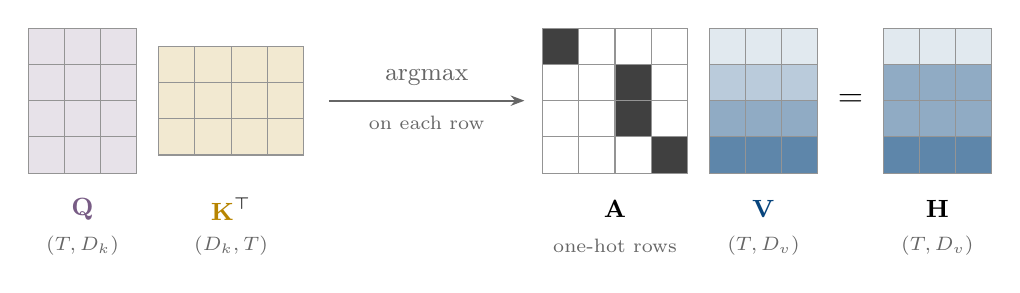
\begin{tikzpicture}[x=0.46cm, y=0.46cm,
            cell/.style={draw=drawgray!70, line width=0.4pt},
            mlab/.style={font=\small},
            slab/.style={font=\scriptsize, text=black!60},
        ]
        % Q (T x D_k)
        \foreach \r in {0,...,3} \foreach \c in {0,...,2}
        \draw[cell, fill=qcolor!18] (\c,-\r) rectangle ++(1,-1);
        \node[mlab] at (1.5,-5) {$\qc{\vc{Q}}$};
        \node[slab] at (1.5,-6) {$(T,D_k)$};
        % K^T (D_k x T)
        \foreach \r in {0,...,2} \foreach \c in {0,...,3}
        \draw[cell, fill=kcolor!18] ({3.6+\c},{-0.5-\r}) rectangle ++(1,-1);
        \node[mlab] at (5.6,-5) {$\kc{\vc{K}}^{\top}$};
        \node[slab] at (5.6,-6) {$(D_k,T)$};
        % argmax arrow
        \draw[-{Stealth[length=5pt]}, drawgray, line width=0.6pt] (8.3,-2) -- (13.7,-2)
        node[midway, above=2pt, font=\small] {$\operatorname{argmax}$}
        node[midway, below=2pt, slab] {on each row};
        % A (T x T), one-hot rows: token t reads the value of key t*
        \def\hot{{0,2,2,3}}
        \foreach \r in {0,...,3} \foreach \c in {0,...,3} {
                \pgfmathtruncatemacro{\h}{\hot[\r]}
                \ifnum\c=\h
                    \draw[cell, fill=black!75] ({14.2+\c},-\r) rectangle ++(1,-1);
                \else
                    \draw[cell, fill=white] ({14.2+\c},-\r) rectangle ++(1,-1);
                \fi
            }
        \node[mlab] at (16.2,-5) {$\vc{A}$};
        \node[slab] at (16.2,-6) {one-hot rows};
        % V (T x D_v), one shade per stored value
        \def\vshade{{12,28,45,65}}
        \foreach \r in {0,...,3} {
                \pgfmathtruncatemacro{\s}{\vshade[\r]}
                \foreach \c in {0,...,2}
                \draw[cell, fill=vcolor!\s] ({18.8+\c},-\r) rectangle ++(1,-1);
            }
        \node[mlab] at (20.3,-5) {$\vcl{\vc{V}}$};
        \node[slab] at (20.3,-6) {$(T,D_v)$};
        \node[font=\large] at (22.7,-2) {$=$};
        % H: each row is a copy of the selected row of V
        \foreach \r in {0,...,3} {
                \pgfmathtruncatemacro{\h}{\hot[\r]}
                \pgfmathtruncatemacro{\s}{\vshade[\h]}
                \foreach \c in {0,...,2}
                \draw[cell, fill=vcolor!\s] ({23.6+\c},-\r) rectangle ++(1,-1);
            }
        \node[mlab] at (25.1,-5) {$\vc{H}$};
        \node[slab] at (25.1,-6) {$(T,D_v)$};
    \end{tikzpicture}

    \vspace{1.5em}
    {\small Each query retrieves the value of its best-matching key, like
        \pythoninline{d[q]}: every row of $\vc{H}$ is a copy of one row of
        $\vcl{\vc{V}}$. Small changes to the scores leave the argmax unchanged, so
        the gradient is zero almost everywhere.\par}

\end{frame}

\begin{frame}{Trainable keys and values}
    \setlength{\parskip}{6pt}

    Consider a variant in which we parameterize explicitly the keys and
    values as trainable matrices $\kc{\vc{K}}\sim(M,D)$ and
    $\vcl{\vc{V}}\sim(M,D_v)$ (ignoring $\vc{W}_q$ and the scaling):
    \[
        \vc{H}=\operatorname{softmax}\left(\vc{X}\kc{\vc{K}}^{\top}\right)\vcl{\vc{V}} \,.
    \]
    The rows of $\kc{\vc{K}}$ and $\vcl{\vc{V}}$ store patterns retrieved by
    an attention-like operation (a \myalert{memory layer}). But this is also a
    \myalert{two-layer MLP} with a softmax activation function: MLPs can be
    seen as attention over trainable keys and values.

    If we remove the softmax, we get a \myalert{linear associative memory}
    $\vc{H}=\vc{X}\vc{S}$, with $\vc{S}=\sum_i\kc{\vc{k}_i}\vcl{\vc{v}_i}^{\top}$.
    Each read returns the matching value plus \myalert{interference} from all
    other pairs, which degrades quickly once $M$ exceeds $D$.

    \SlideSource{Geva et al. (2021), \textit{Transformer feed-forward layers are key-value memories}, EMNLP; A. Wang (2026), \href{https://alexwang.ai/posts/associative-memory/}{\textit{You could have invented transformers from memory}}, blog post.}

\end{frame}

\begin{frame}{Causal self-attention}
    \setlength{\parskip}{6pt}

    For next-token prediction, $\vc{h}_t$ must not depend on tokens after $t$,
    \NNDSorNN{as with causal convolutions}{as in a recurrent model}. We add a \myalert{mask} to the scores before
    the softmax:
    \[
        \vc{H}=\operatorname{softmax}\left(\frac{\qc{\vc{Q}}\kc{\vc{K}}^{\top}}{\sqrt{D_k}}
        +\eqnmarkbox[drawblue]{mask}{\vc{M}}\right)\vcl{\vc{V}},
        \qquad
        \idx{\vc{M}}{t,t'}=\begin{cases}0 & t'\le t\\ -\infty & t'>t\end{cases}
    \]
    \annotate[yshift=-0.8em]{below,left}{mask}{causal mask}
    \vspace{0.6em}

    Since $\exp(-\infty)=0$, future tokens get zero weight and each row still
    sums to one. In code, $-\infty$ is a large negative number, or the scores
    are filled in place.

    This is the single difference between our decoder and an encoder: without
    $\vc{M}$, every token sees the whole sequence.

\end{frame}

\begin{frame}{Visualizing the causal mask}
    \centering
    \vspace{1em}
    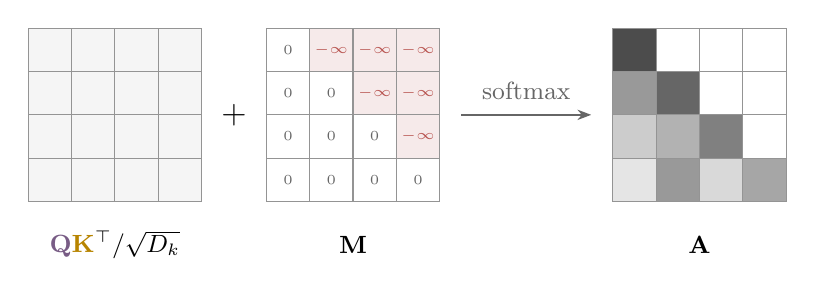
\begin{tikzpicture}[x=0.55cm, y=0.55cm,
            cell/.style={draw=drawgray!70, line width=0.4pt},
            mlab/.style={font=\small},
            inf/.style={font=\tiny, text=drawred},
        ]
        % Scores
        \foreach \r in {0,...,3} \foreach \c in {0,...,3}
        \draw[cell, fill=drawgray_l] (\c,-\r) rectangle ++(1,-1);
        \node[mlab] at (2,-5) {$\qc{\vc{Q}}\kc{\vc{K}}^{\top}/\sqrt{D_k}$};
        \node[font=\large] at (4.75,-2) {$+$};
        % Mask
        \foreach \r in {0,...,3} \foreach \c in {0,...,3} {
                \ifnum\c>\r
                    \draw[cell, fill=drawred!12] ({5.5+\c},-\r) rectangle ++(1,-1);
                    \node[inf] at ({6+\c},{-\r-0.5}) {$-\infty$};
                \else
                    \draw[cell, fill=white] ({5.5+\c},-\r) rectangle ++(1,-1);
                    \node[font=\tiny, text=black!60] at ({6+\c},{-\r-0.5}) {$0$};
                \fi
            }
        \node[mlab] at (7.5,-5) {$\vc{M}$};
        % softmax arrow
        \draw[-{Stealth[length=5pt]}, drawgray, line width=0.6pt] (10,-2) -- (13,-2)
        node[midway, above=2pt, font=\small] {softmax};
        % Causal attention matrix
        \def\arow{{70},{40,60},{20,30,50},{10,40,15,35}}
        \foreach \r in {0,...,3} \foreach \c in {0,...,3}
        \draw[cell, fill=white] ({13.5+\c},-\r) rectangle ++(1,-1);
        \foreach \row [count=\r from 0] in \arow {
            \foreach \v [count=\c from 0] in \row {
                \draw[cell, fill=black!\v] ({13.5+\c},-\r) rectangle ++(1,-1);
            }
        }
        \node[mlab] at (15.5,-5) {$\vc{A}$};
    \end{tikzpicture}

    \vspace{1.5em}
    {\small Adding $-\infty$ above the diagonal gives future tokens exactly zero
        weight. Multiplying the scores by a $0/1$ mask would not work, since
        $\exp(0)=1$; zeroing $\vc{A}$ after the softmax would break the sum to
        one.\par}

\end{frame}

\subsection{Multi-head attention}

\begin{frame}{Multi-head attention}
    \setlength{\parskip}{6pt}

    The SA layer can handle quasi-sparse dependencies (because of the
    softmax), and also dynamic ones (because of the attention function).
    However, what happens when a token depends on multiple subsets of tokens?

    A common generalization in this case is \myalert{multi-head attention}
    (MHA). It works by computing $i=1,\ldots,h$ separate sets of queries,
    keys, and values:
    \[
        \qc{\vc{Q}_i=\vc{X}\vc{W}_{q,i}}, \qquad
        \kc{\vc{K}_i=\vc{X}\vc{W}_{k,i}}, \qquad
        \vcl{\vc{V}_i=\vc{X}\vc{W}_{v,i}},
    \]
    \[
        \vc{H}_i=\operatorname{softmax}\left(\frac{\qc{\vc{Q}_i}\kc{\vc{K}_i}^{\top}}{\sqrt{D_k}}\right)\vcl{\vc{V}_i} \,.
    \]
    Each set is a \myalert{head}, with its own attention matrix $\vc{A}_i$,
    so different heads can attend to different tokens. We now have $3h$
    trainable matrices.

\end{frame}

\begin{frame}{Combining the heads}
    \setlength{\parskip}{6pt}

    The previous operation has $h$ separate outputs; we combine them by
    concatenation over the embedding dimension, and a final reprojection with
    a trainable output matrix $\vc{W}_o$:
    \[
        \shape{\vc{H}}{(T,D)}
        =\eqnmarkbox[drawblue]{cat}{\begin{bmatrix}\vc{H}_1 & \cdots & \vc{H}_h\end{bmatrix}}
        \vc{W}_o \,,
        \qquad \vc{W}_o\sim(hD_v,D) \,.
    \]
    \annotate[yshift=-0.8em]{below,right}{cat}{$(T,hD_v)$}
    \vspace{0.8em}

    As hyperparameters, we typically choose the embedding dimension $D$ and
    the number of heads $h$, and we set $D_k=D_v=D/h$ for all heads. The
    output has the same shape as the input, so MHA layers can be stacked.

    With $D_k=D_v=D/h$, the four projections hold \myalert{$4D^2$ parameters
        for any $h$}: more heads split the same budget into smaller subspaces.

\end{frame}

\begin{frame}{Visualizing multi-head attention}
    \centering
    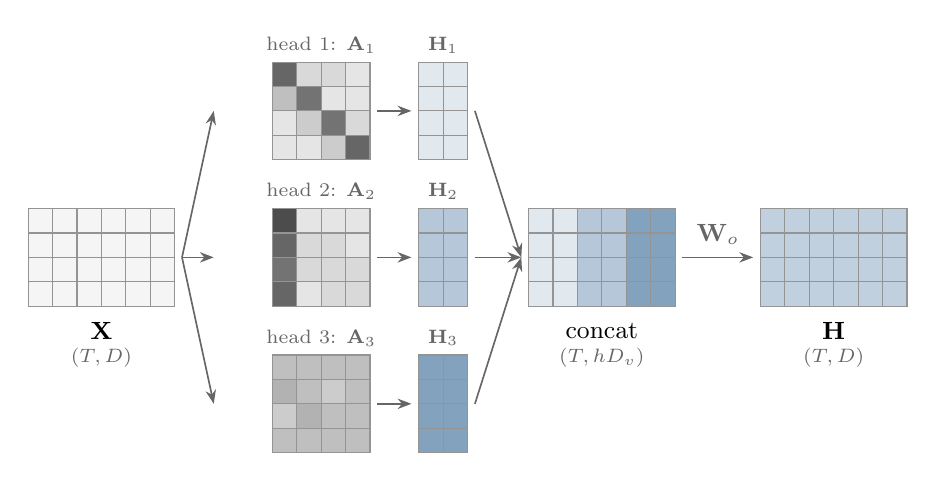
\begin{tikzpicture}[x=0.31cm, y=0.31cm,
            cell/.style={draw=drawgray!70, line width=0.4pt},
            mlab/.style={font=\small},
            slab/.style={font=\scriptsize, text=black!60},
            arr/.style={tfarr},
        ]
        % X (T x D)
        \foreach \r in {0,...,3} \foreach \c in {0,...,5}
        \draw[cell, fill=drawgray_l] (\c,-\r) rectangle ++(1,-1);
        \node[mlab] at (3,-5) {$\vc{X}$};
        \node[slab] at (3,-6.1) {$(T,D)$};
        % Heads: attention matrices and outputs
        \foreach \hy/\hname/\pat/\shade in {
        6/1/{{60,15,15,10},{25,55,10,10},{10,20,55,15},{10,10,20,60}}/12,
        0/2/{{70,10,10,10},{60,15,15,10},{55,15,15,15},{60,10,15,15}}/30,
        -6/3/{{25,25,25,25},{30,25,20,25},{20,30,25,25},{25,25,25,25}}/50} {
        \begin{scope}[yshift=\hy*0.31cm]
            \foreach \row [count=\r from 0] in \pat {
                \foreach \v [count=\c from 0] in \row {
                    \draw[cell, fill=black!\v] ({10+\c},-\r) rectangle ++(1,-1);
                }
            }
            \node[slab] at (12,0.7) {head \hname: $\vc{A}_{\hname}$};
            \foreach \r in {0,...,3} \foreach \c in {0,1}
            \draw[cell, fill=vcolor!\shade] ({16+\c},-\r) rectangle ++(1,-1);
            \node[slab] at (17,0.7) {$\vc{H}_{\hname}$};
            \draw[arr] (14.3,-2) -- (15.7,-2);
        \end{scope}
        \draw[arr] (6.3,-2) -- (7.6,{\hy-2});
        \draw[arr] (18.3,{\hy-2}) -- (20.2,-2);
        }
        % Concatenation
        \foreach \c/\shade in {0/12,1/12,2/30,3/30,4/50,5/50}
        \foreach \r in {0,...,3}
        \draw[cell, fill=vcolor!\shade] ({20.5+\c},-\r) rectangle ++(1,-1);
        \node[mlab] at (23.5,-5) {concat};
        \node[slab] at (23.5,-6.1) {$(T,hD_v)$};
        \draw[arr] (26.8,-2) -- (29.7,-2) node[midway, above=1pt, font=\small] {$\vc{W}_o$};
        % H (T x D)
        \foreach \r in {0,...,3} \foreach \c in {0,...,5}
        \draw[cell, fill=vcolor!25] ({30+\c},-\r) rectangle ++(1,-1);
        \node[mlab] at (33,-5) {$\vc{H}$};
        \node[slab] at (33,-6.1) {$(T,D)$};
    \end{tikzpicture}

    \vspace{1em}
    {\small Three heads with $D_v=D/3$: each has its own attention pattern
        (here local, on the first token, and almost uniform). $\vc{W}_o$ mixes
        the concatenated outputs back into $D$ features.\par}

\end{frame}

\begin{frame}[fragile]{Attention in code}
    \setlength{\parskip}{5pt}

    \begin{python}[gobble=8,aboveskip=2pt,belowskip=4pt]
        def mha(x, Wq, Wk, Wv, Wo, h):                    # x: (B, T, D)
            B, T, D = x.shape
            def heads(y):                                 # (B, h, T, D/h)
                return y.view(B, T, h, D // h).transpose(1, 2)
            q, k, v = heads(x @ Wq), heads(x @ Wk), heads(x @ Wv)
            s = q @ k.transpose(-2, -1) / (D // h) ** 0.5 # (B, h, T, T)
            mask = torch.ones(T, T, dtype=torch.bool).triu(1)
            a = s.masked_fill(mask, float('-inf')).softmax(-1)
            out = (a @ v).transpose(1, 2).reshape(B, T, D) # concat heads
            return out @ Wo
    \end{python}

    This \myalert{naive} implementation of causal MHA stores all the attention
    matrices, $(B,h,T,T)$ numbers. PyTorch's
    \pythoninline{F.scaled_dot_product_attention} (with
    \pythoninline{is_causal=True}) gives the same result computing $\vc{A}$
    block by block, without storing it\NNDSorNN{ (next lecture)}{}.

\end{frame}

\subsection{The transformer block}

\begin{frame}{The transformer block}
    \setlength{\parskip}{6pt}

    In transformers, the MHA layer is always used inside a more complex block,
    called the \myalert{transformer block}. Originally, this was composed of an
    MHA layer, two layer normalization operations, two residual connections,
    and a so-called \myalert{position-wise} network as follows:
    \begin{enumerate}
        \item Start with an MHA layer: $\vc{H}=\operatorname{MHA}(\vc{X})$.
        \item Add a residual connection and a layer normalization operation:
              $\vc{H}=\operatorname{LayerNorm}(\vc{H}+\vc{X})$.
        \item Apply an MLP $g$ on each row: $\vc{F}=g(\vc{H})$.
        \item Do again step 2: $\vc{H}=\operatorname{LayerNorm}(\vc{F}+\vc{H})$.
    \end{enumerate}

    The output has shape $(T,D)$ like the input: a transformer is a stack of
    these blocks.

    \SlideSource{Vaswani et al. (2017), \textit{Attention is all you need}, NeurIPS.}

\end{frame}

\begin{frame}{Design of the block}
    \setlength{\parskip}{6pt}

    The design of the block was mostly based on empirical considerations.
    Roughly speaking, steps (1)--(2) correspond to a \myalert{token mixing}
    operation, while steps (3)--(4) are a per-token update\NNDSorNN{ which is akin to a
        $1\times1$ convolution}{, with the same MLP applied to every token}.

    \begin{columns}[T,onlytextwidth]
        \begin{column}{0.49\textwidth}
            \begin{tcolorbox}[nndsblue,courseheight={tf-mixing}{0.27\textheight}]
                \textbf{\color{darkcerulean}Token mixing (MHA)}

                Combines rows of $\vc{X}$, with weights that depend on the input.
            \end{tcolorbox}
        \end{column}
        \begin{column}{0.49\textwidth}
            \begin{tcolorbox}[nndsgreen,courseheight={tf-mixing}{0.27\textheight}]
                \textbf{\color{darkgreen}Channel mixing (MLP)}

                Combines the features of each row, with the same weights for every token.
            \end{tcolorbox}
        \end{column}
    \end{columns}

    \medskip
    \NNDSorNN{The block is similar in spirit to a depthwise separable convolution
        (spatial mixing and channel mixing in the CNN lecture). }{}The intermediate
    MLP has two layers, with hidden dimension an integer multiple of $D$
    ($4D$ in the original model).

    \SlideSource{Vaswani et al. (2017), \textit{Attention is all you need}, NeurIPS.}

\end{frame}

\begin{frame}{Pre- and post-normalized blocks}
    \setlength{\parskip}{5pt}

    \centering
    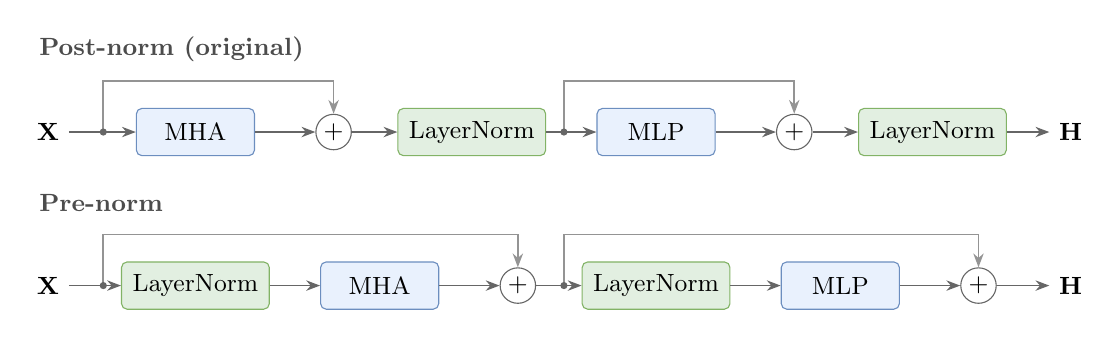
\begin{tikzpicture}[x=1.17cm, y=1cm,
            pb/.style={tfblk, minimum width=1.5cm, minimum height=0.6cm},
            pn/.style={tfnorm, minimum width=1.5cm, minimum height=0.6cm},
            skip/.style={tfarr, drawgray!70},
            ttl/.style={font=\small\bfseries, anchor=west, text=black!70},
        ]
        % Post-norm (original): X -> MHA -> + -> LN -> MLP -> + -> LN
        \node[ttl] at (-0.2,1.05) {Post-norm (original)};
        \node[font=\small] (x) at (0,0) {$\vc{X}$};
        \node[pb] (a) at (1.6,0) {MHA};
        \node[tfsum] (m1) at (3.1,0) {$+$};
        \node[pn] (n1) at (4.6,0) {LayerNorm};
        \node[pb] (f) at (6.6,0) {MLP};
        \node[tfsum] (m2) at (8.1,0) {$+$};
        \node[pn] (n2) at (9.6,0) {LayerNorm};
        \node[font=\small] (y) at (11.1,0) {$\vc{H}$};
        \draw[tfarr] (x) -- (a); \draw[tfarr] (a) -- (m1); \draw[tfarr] (m1) -- (n1);
        \draw[tfarr] (n1) -- (f); \draw[tfarr] (f) -- (m2); \draw[tfarr] (m2) -- (n2);
        \draw[tfarr] (n2) -- (y);
        \draw[skip] (0.6,0) -- (0.6,0.65) -| (m1);
        \draw[skip] (5.6,0) -- (5.6,0.65) -| (m2);
        \fill[drawgray] (0.6,0) circle (1.3pt); \fill[drawgray] (5.6,0) circle (1.3pt);

        % Pre-norm: X -> LN -> MHA -> + -> LN -> MLP -> +
        \begin{scope}[yshift=-1.95cm]
            \node[ttl] at (-0.2,1.05) {Pre-norm};
            \node[font=\small] (x) at (0,0) {$\vc{X}$};
            \node[pn] (n1) at (1.6,0) {LayerNorm};
            \node[pb] (a) at (3.6,0) {MHA};
            \node[tfsum] (m1) at (5.1,0) {$+$};
            \node[pn] (n2) at (6.6,0) {LayerNorm};
            \node[pb] (f) at (8.6,0) {MLP};
            \node[tfsum] (m2) at (10.1,0) {$+$};
            \node[font=\small] (y) at (11.1,0) {$\vc{H}$};
            \draw[tfarr] (x) -- (n1); \draw[tfarr] (n1) -- (a); \draw[tfarr] (a) -- (m1);
            \draw[tfarr] (m1) -- (n2); \draw[tfarr] (n2) -- (f); \draw[tfarr] (f) -- (m2);
            \draw[tfarr] (m2) -- (y);
            \draw[skip] (0.6,0) -- (0.6,0.65) -| (m1);
            \draw[skip] (5.6,0) -- (5.6,0.65) -| (m2);
            \fill[drawgray] (0.6,0) circle (1.3pt); \fill[drawgray] (5.6,0) circle (1.3pt);
        \end{scope}
    \end{tikzpicture}
    \par\vspace{0.6em}
    \justifying

    The original block is called \myalert{post-normalized}. A
    \myalert{pre-normalized} variant is also common due to it being simpler to
    train in most cases: $\vc{H}=\vc{X}+\operatorname{MHA}(\operatorname{LayerNorm}(\vc{X}))$.

    The skip path carries $\vc{X}$, and the gradient, unchanged through all
    blocks. In post-norm, the gradient crosses every LayerNorm, and training
    needs a small learning rate in the first steps (\myalert{warmup}).

    \SlideSource{Xiong et al. (2020), \textit{On layer normalization in the transformer architecture}, ICML.}

\end{frame}

\subsection{Positional embeddings}

\begin{frame}{Permutation matrices}
    \setlength{\parskip}{6pt}

    In text, the $t$-th row of $\vc{X}$ represents a single token. To reason
    about reordering the tokens, we use permutation matrices.

    A \myalert{permutation matrix} $\vc{P}\sim(T,T)$ has exactly one $1$ in
    each row and in each column, and zeros elsewhere. Multiplying
    $\vc{P}\vc{X}$ reorders the rows of $\vc{X}$.

    For example:
    \[
        \vc{P}=\begin{bmatrix}1&0&0\\0&0&1\\0&1&0\end{bmatrix},
        \qquad
        \vc{P}\begin{bmatrix}\vc{x}_0^{\top}\\\vc{x}_1^{\top}\\\vc{x}_2^{\top}\end{bmatrix}
        =\begin{bmatrix}\vc{x}_0^{\top}\\\vc{x}_2^{\top}\\\vc{x}_1^{\top}\end{bmatrix}.
    \]
    Multiplying on the right, $\vc{A}\vc{P}^{\top}$, reorders the columns in
    the same way. Since $\vc{P}^{\top}$ undoes the permutation,
    $\vc{P}^{\top}\vc{P}=\vc{I}$.

\end{frame}

\begin{frame}{The MHA layer is equivariant to permutations}
    \setlength{\parskip}{5pt}
    \setlength{\abovedisplayskip}{4pt}\setlength{\belowdisplayskip}{4pt}

    Without the causal mask, the MHA layer is \textit{equivariant} to the
    ordering of the tokens:
    \[
        \operatorname{MHA}(\vc{P}\vc{X})=\vc{P}\cdot\operatorname{MHA}(\vc{X}) \,.
    \]
    Follow one head (scaling omitted). The projections become
    $\vc{P}\qc{\vc{Q}}$, $\vc{P}\kc{\vc{K}}$, $\vc{P}\vcl{\vc{V}}$, and the
    scores $\vc{P}\qc{\vc{Q}}\kc{\vc{K}}^{\top}\vc{P}^{\top}$ have rows and
    columns reordered in the same way. A row-wise softmax does not care about
    this reordering, so:
    \[
        \operatorname{softmax}(\vc{P}\qc{\vc{Q}}\kc{\vc{K}}^{\top}\vc{P}^{\top})\,\vc{P}\vcl{\vc{V}}
        =\vc{P}\operatorname{softmax}(\qc{\vc{Q}}\kc{\vc{K}}^{\top})\,\eqnmarkbox[drawblue]{ptp}{\vc{P}^{\top}\vc{P}}\,\vcl{\vc{V}}
        =\vc{P}\vc{H} \,.
    \]
    \annotate[yshift=-0.6em]{below,right}{ptp}{$=\vc{I}$}
    \vspace{0.6em}

    Concatenation and $\vc{W}_o$, like the MLP and LayerNorm, act on each row,
    so the same holds trivially for the entire block. This is not a good
    property to have for sequences.

    The causal mask breaks the symmetry: token $t$ sees exactly $t+1$ tokens.

\end{frame}

\begin{whiteframe}{Visualizing permutation equivariance}

    \begin{figure}
        \centering
        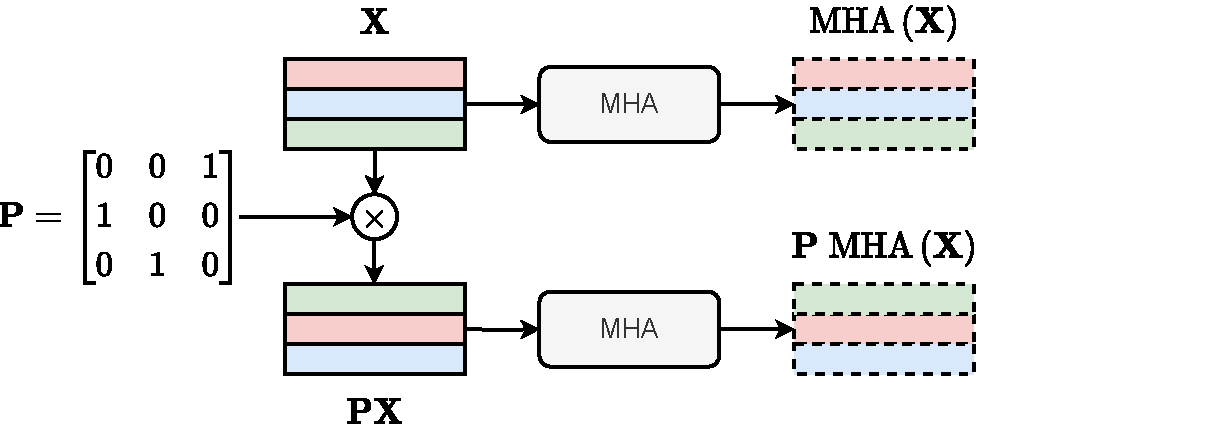
\includegraphics[width=0.8\columnwidth]{images/transformers/book/PermutationEquivariance}
    \end{figure}

    {\small Permuting the input rows permutes the output rows in the same way.
    Each output depends on which tokens are present, not on their order: without
    positions, ``dog'' gets the same vector in ``the dog bit the man'' and
    ``the man bit the dog''.\par}

\end{whiteframe}

\begin{frame}{Positional embeddings}
    \setlength{\parskip}{6pt}

    Before the first block, we sum (or concatenate) to the input $\vc{X}$ a
    matrix of \myalert{positional embeddings} $\vc{E}\sim(T,D)$:
    \[
        \vc{X}'=\vc{X}+\vc{E} \,,
    \]
    where each row $\idx{\vc{E}}{t,:}$ should \textit{uniquely} encode the
    position $t$. Using this strategy, we `break' the equivariance.

    \begin{figure}
        \centering
        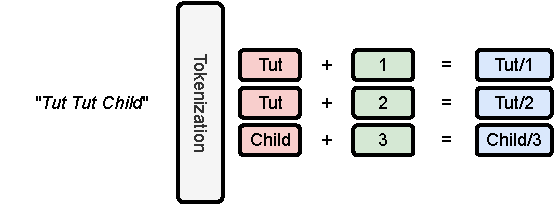
\includegraphics[width=0.5\columnwidth]{images/transformers/book/positional_embeddings}
    \end{figure}
    {\small The same token at two different positions is now represented by
    different vectors.\par}

\end{frame}

\begin{frame}{Trainable positional embeddings}
    \setlength{\parskip}{6pt}

    The simplest choice is to \textit{learn} the positional embeddings with an
    embedding layer (\texttt{nn.Embedding}), as for the tokens:
    \begin{itemize}
        \item To each position $t$ we associate an embedding vector of
              dimension $D$.
        \item The embeddings are trained with the rest of the network.
    \end{itemize}
    This is the strategy of BERT, GPT-2 and the Vision Transformer.

    However, we need to fix the maximum length $T_{\max}$, and positions never
    seen in training have no embedding. To change the image resolution, ViT
    interpolates the trained embeddings.

\end{frame}

\begin{frame}{Sinusoidal embeddings}

    \begin{columns}[c,onlytextwidth]
        \begin{column}{0.55\textwidth}%
            \small\setlength{\parskip}{5pt}%
            \RaggedRight\setlength{\parindent}{0pt}%
            A sinusoid $\sin(\omega t)$ is a clock with frequency $\omega$:
            it gives the position only modulo its period.

            With multiple frequencies, we get a clock with $D$ hands, each
            rotating at its own speed:
            \[
                \idx{\vc{E}}{t,j}=\sin(\omega_j t),
                \qquad \omega_j=\frac{1}{b^{j/D}} \,.
            \]
            The frequencies decrease geometrically, from a period of $2\pi$
            tokens ($j=0$) to about $b\cdot 2\pi$. The \myalert{base} $b$ is
            a hyperparameter, larger than the longest sequence.

            No parameters, and no maximum length fixed \textit{a priori}.
        \end{column}
        \begin{column}{0.42\textwidth}
            \centering
            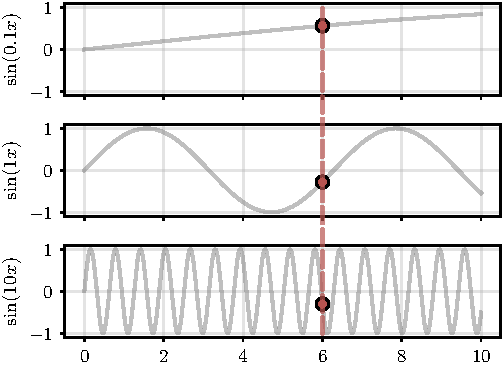
\includegraphics[width=\linewidth]{images/transformers/book/positional_embeddings_plot}
            \par{\scriptsize Three hands at one position (red line).\par}
        \end{column}
    \end{columns}

\end{frame}

\begin{frame}{Sines and cosines}
    \setlength{\parskip}{3pt}
    \setlength{\abovedisplayskip}{4pt}\setlength{\belowdisplayskip}{4pt}

    The original transformer alternates sines and cosines of the same
    frequency, with $\omega_j=b^{-2j/D}$ and $b=10000$:
    \[
        \idx{\vc{E}}{t,2j}=\sin(\omega_j t), \qquad
        \idx{\vc{E}}{t,2j+1}=\cos(\omega_j t) \,.
    \]
    Each pair is a point on a circle. Moving by $p$ positions rotates it by
    the angle $\omega_j p$, whatever $t$ is:
    \[
        \idx{\vc{E}}{t+p,:}=\idx{\vc{E}}{t,:}\,\vc{T}(p),
        \qquad
        \vc{T}(p)=\operatorname{diag}\big(\vc{R}(\omega_0p),\ldots\big),
        \quad
        \vc{R}(\theta)=\begin{bmatrix}\cos\theta&-\sin\theta\\\sin\theta&\cos\theta\end{bmatrix}.
    \]

    Hence $\idx{\vc{E}}{t,:}\idx{\vc{E}}{t+p,:}^{\top}=\sum_j\cos(\omega_jp)$
    depends only on $p$. Rotating queries and keys gives \myalert{rotary
        embeddings} (RoPE), shortly.

    \SlideSource{Vaswani et al. (2017), \textit{Attention is all you need}, NeurIPS.}

\end{frame}

\begin{frame}{Relative positional embeddings}
    \setlength{\parskip}{6pt}

    Another possibility is \myalert{relative positional embeddings}: we
    modify the attention function to make it depend on the distance $t-t'$
    between tokens, as in the weight $\alpha(\vc{x}_t,\vc{x}_{t'},t'-t)$ of
    non-local networks. Nothing is added to $\vc{X}$, and position enters
    every attention layer.

    \begin{columns}[T,onlytextwidth]
        \begin{column}{0.49\textwidth}
            \begin{tcolorbox}[nndsblue,courseheight={tf-relative}{0.3\textheight}]
                \textbf{\color{darkcerulean}Rotate queries and keys}

                Rotary embeddings (RoPE): Llama, Qwen, Gemma, Mistral, and most
                current language models.
            \end{tcolorbox}
        \end{column}
        \begin{column}{0.49\textwidth}
            \begin{tcolorbox}[nndsgreen,courseheight={tf-relative}{0.3\textheight}]
                \textbf{\color{darkgreen}Add a bias to the scores}

                Linear biases (ALiBi, used in BLOOM and MPT), or the learned
                biases of T5.
            \end{tcolorbox}
        \end{column}
    \end{columns}

\end{frame}

\begin{frame}{Rotary positional embeddings (RoPE)}
    \setlength{\parskip}{6pt}

    RoPE splits each query and key into $D_k/2$ pairs of components, and
    treats every pair as a point in the plane. Pair $j$ of the query (and of
    the key) at position $t$ is rotated by an angle proportional to $t$:
    \[
        \qc{\begin{bmatrix}\tilde{q}_{t,2j}\\\tilde{q}_{t,2j+1}\end{bmatrix}}
        =\vc{R}(\omega_jt)\qc{\begin{bmatrix}q_{t,2j}\\q_{t,2j+1}\end{bmatrix}},
        \qquad
        \vc{R}(\theta)=\begin{bmatrix}\cos\theta&-\sin\theta\\\sin\theta&\cos\theta\end{bmatrix}.
    \]
    \vspace{0.3em}

    \begin{columns}[T,onlytextwidth]
        \begin{column}{0.49\textwidth}
            \begin{tcolorbox}[nndsblue,boxsep=1mm,top=1mm,bottom=1mm,courseheight={tf-rope}{0.17\textheight}]
                \small
                \textbf{\color{darkcerulean}Why pairs?}\par
                A rotation needs two dimensions. It keeps the norm, and two
                rotations add their angles.
            \end{tcolorbox}
        \end{column}
        \begin{column}{0.49\textwidth}
            \begin{tcolorbox}[nndsgreen,boxsep=1mm,top=1mm,bottom=1mm,courseheight={tf-rope}{0.17\textheight}]
                \small
                \textbf{\color{darkgreen}Why many frequencies?}\par
                One pair is a clock with one hand. With
                $\omega_j=b^{-2j/D_k}$, fast pairs separate nearby tokens,
                slow pairs distant ones.
            \end{tcolorbox}
        \end{column}
    \end{columns}

    \SlideSource{Su et al. (2024), \textit{RoFormer: Enhanced transformer with rotary position embedding}, Neurocomputing.}

\end{frame}

\begin{frame}{Visualizing RoPE}
    \centering
    \vspace{0.5em}
    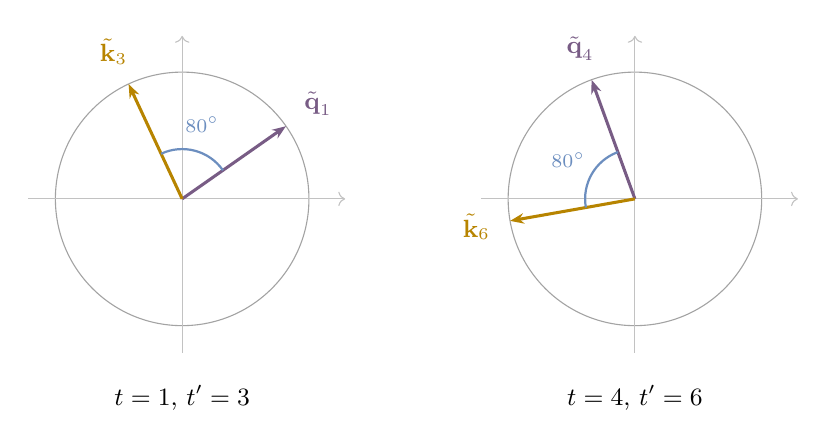
\begin{tikzpicture}[scale=1.15,
        vec/.style={-{Stealth[length=5pt]}, line width=1.1pt},
        lab/.style={font=\small},
        ]
        \foreach \x/\t/\tp/\qa/\ka in {0/1/3/35/115, 5/4/6/110/190} {
                \begin{scope}[xshift=\x cm]
                    \draw[drawgray!60] (0,0) circle (1.4);
                    \draw[drawgray!40, ->] (-1.7,0) -- (1.8,0);
                    \draw[drawgray!40, ->] (0,-1.7) -- (0,1.8);
                    \draw[vec, qcolor] (0,0) -- (\qa:1.4)
                    node[lab, anchor=\qa+180, shift={(\qa:0.12)}] {$\qc{\tilde{\vc{q}}_{\t}}$};
                    \draw[vec, kcolor] (0,0) -- (\ka:1.4)
                    node[lab, anchor=\ka+180, shift={(\ka:0.12)}] {$\kc{\tilde{\vc{k}}_{\tp}}$};
                    \draw[drawblue, thick] (\qa:0.55) arc (\qa:\ka:0.55);
                    \node[font=\scriptsize, text=drawblue] at ({(\qa+\ka)/2}:0.85) {$80^\circ$};
                    \node[lab] at (0,-2.2) {$t=\t$, $t'=\tp$};
                \end{scope}
            }
    \end{tikzpicture}

    \vspace{1em}
    {\small One pair of components, rotating by $25^\circ$ per position. Moving
        both tokens by three positions rotates both vectors: the angle between
        them, hence the score, does not change.\par}

\end{frame}

\begin{frame}{RoPE for all pairs}
    \setlength{\parskip}{5pt}

    Collecting the rotations of all pairs in a block-diagonal matrix:
    \[
        \qc{\tilde{\vc{q}}_t=\vc{R}_t\vc{q}_t}, \qquad
        \kc{\tilde{\vc{k}}_{t'}=\vc{R}_{t'}\vc{k}_{t'}}, \qquad
        \vc{R}_t=\operatorname{diag}\big(\vc{R}(\omega_0t),\ldots,\vc{R}(\omega_{D_k/2-1}t)\big) \,.
    \]
    Rotations compose, $\vc{R}_t^{\top}\vc{R}_{t'}=\vc{R}_{t'-t}$, so the
    score becomes:
    \vspace{0.8em}
    \[
        s_{t,t'}=\frac{\qc{\tilde{\vc{q}}_t^{\top}}\kc{\tilde{\vc{k}}_{t'}}}{\sqrt{D_k}}
        =\frac{\qc{\vc{q}_t^{\top}}\eqnmarkbox[drawblue]{rot}{\vc{R}_{t'-t}}\kc{\vc{k}_{t'}}}{\sqrt{D_k}} \,.
    \]
    \annotate[yshift=0.6em]{above,right}{rot}{position enters only through $t'-t$}

    The values are not rotated, nothing is added to $\vc{X}$, and there are no
    parameters.

\end{frame}

\begin{frame}[fragile]{RoPE in code}
    \setlength{\parskip}{5pt}

    \begin{python}[gobble=8,aboveskip=4pt,belowskip=4pt]
        def rope(x, base=10000.0):                     # x: (..., T, D_k)
        T, D = x.shape[-2:]
        w = base ** (-torch.arange(0, D, 2) / D)   # (D_k/2,) frequencies
        ang = torch.arange(T)[:, None] * w         # (T, D_k/2) angles
        cos, sin = ang.cos(), ang.sin()
        x1, x2 = x[..., 0::2], x[..., 1::2]        # the pairs
        return torch.stack([x1 * cos - x2 * sin,
                x1 * sin + x2 * cos], -1).flatten(-2)

        scores = rope(q) @ rope(k).transpose(-2, -1) / D_k ** 0.5
    \end{python}

    RoPE is applied in every attention layer, after the projections and
    before the scores. The base $b$ sets the slowest rotation: recent models
    raise it (Llama~3 uses \mbox{$b=500{,}000$}) to cover longer contexts.

\end{frame}

\begin{frame}{Attention with linear biases (ALiBi)}
    \setlength{\parskip}{6pt}

    \myalert{ALiBi} adds no embedding to $\vc{X}$; it subtracts from the
    scores a penalty proportional to the distance:
    \[
        s_{t,t'}=\frac{\qc{\vc{q}_t^{\top}}\kc{\vc{k}_{t'}}}{\sqrt{D_k}}
        -\eqnmarkbox[drawblue]{slope}{m_i}\,(t-t'),
        \qquad t'\le t \,.
    \]
    \annotate[yshift=-0.8em]{below,right}{slope}{fixed slope of head $i$ (e.g., $1/2, 1/4, \ldots$)}
    \vspace{0.6em}

    The penalty is not trained. Heads with a large slope look at nearby
    tokens, heads with a small one at the whole past. Models trained on short
    sequences still work on longer ones.

    \SlideSource{Press et al. (2022), \textit{Train short, test long: Attention with linear biases enables input length extrapolation}, ICLR.}

\end{frame}

\begin{frame}{Visualizing ALiBi}
    \centering
    \vspace{0.5em}
    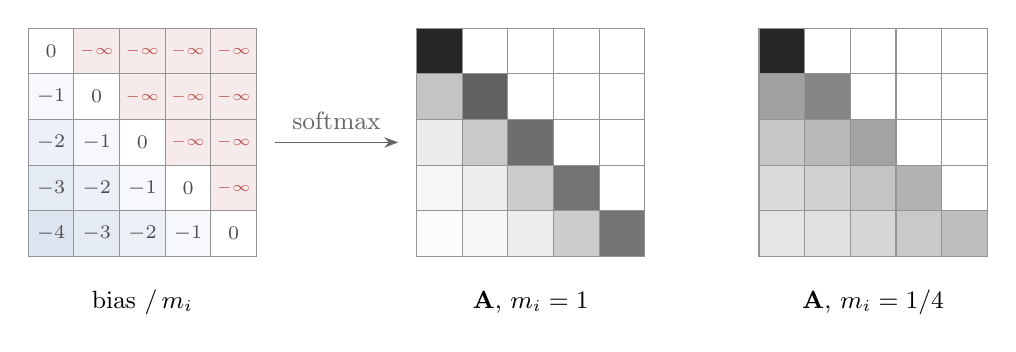
\begin{tikzpicture}[x=0.58cm, y=0.58cm,
            cell/.style={draw=drawgray!70, line width=0.4pt},
            mlab/.style={font=\small},
            num/.style={font=\scriptsize, text=black!70},
            inf/.style={font=\tiny, text=drawred},
        ]
        % Bias matrix: -(t - t') below the diagonal, -inf above
        \foreach \r in {0,...,4} \foreach \c in {0,...,4} {
                \ifnum\c>\r
                    \draw[cell, fill=drawred!12] (\c,-\r) rectangle ++(1,-1);
                    \node[inf] at ({\c+0.5},{-\r-0.5}) {$-\infty$};
                \else
                    \pgfmathtruncatemacro{\d}{\r-\c}
                    \pgfmathtruncatemacro{\sh}{6*\d}
                    \draw[cell, fill=drawblue!\sh] (\c,-\r) rectangle ++(1,-1);
                    \node[num] at ({\c+0.5},{-\r-0.5}) {$\ifnum\d=0 0\else -\d\fi$};
                \fi
            }
        \node[mlab] at (2.5,-6) {bias $/\,m_i$};
        % Two heads
        \foreach \x/\m/\rows in {
        8.5/{m_i=1}/{{85},{23,62},{8,21,57},{3,7,20,55},{1,3,7,20,54}},
        16/{m_i=1/4}/{{85},{37,48},{22,28,36},{14,18,23,30},{10,12,16,21,26}}} {
        \foreach \r in {0,...,4} \foreach \c in {0,...,4}
        \draw[cell, fill=white] ({\x+\c},-\r) rectangle ++(1,-1);
        \foreach \row [count=\r from 0] in \rows {
            \foreach \v [count=\c from 0] in \row {
                \draw[cell, fill=black!\v] ({\x+\c},-\r) rectangle ++(1,-1);
            }
        }
        \node[mlab] at ({\x+2.5},-6) {$\vc{A}$, $\m$};
        }
        \draw[-{Stealth[length=5pt]}, drawgray, line width=0.6pt] (5.4,-2.5) -- (8.1,-2.5)
        node[midway, above=1pt, font=\small] {softmax};
    \end{tikzpicture}

    \vspace{1.2em}
    {\small Attention weights when all the scores $\qc{\vc{q}_t^{\top}}\kc{\vc{k}_{t'}}$
        are equal. A large slope gives a soft local window, a small one an
        almost uniform average over the past.\par}

\end{frame}

\begin{frame}{No positional embeddings (NoPE)}
    \setlength{\parskip}{6pt}

    In a decoder, the causal mask already breaks the equivariance: token $t$
    attends to exactly $t+1$ tokens. For example, a head with equal scores
    outputs $\vc{h}_t=\frac{1}{t+1}\sum_{t'\le t}\vcl{\vc{v}_{t'}}$, where the
    contribution of the first token shrinks as $1/(t+1)$: later layers can
    read the position from it.

    Causal language models with \myalert{no positional embeddings} (NoPE)
    train almost as well as with them, and degrade less on sequences longer
    than those seen in training.

    This only works for decoders: without the mask, an encoder with no
    positional embeddings is still equivariant.

    \SlideSource{Haviv et al. (2022), \textit{Transformer language models without positional encodings still learn positional information}, Findings of EMNLP;
        Kazemnejad et al. (2023), \textit{The impact of positional encoding on length generalization in transformers}, NeurIPS.}

\end{frame}

\begin{frame}{Interleaving RoPE and NoPE}
    \setlength{\parskip}{6pt}

    \centering
    \vspace{0.3em}
    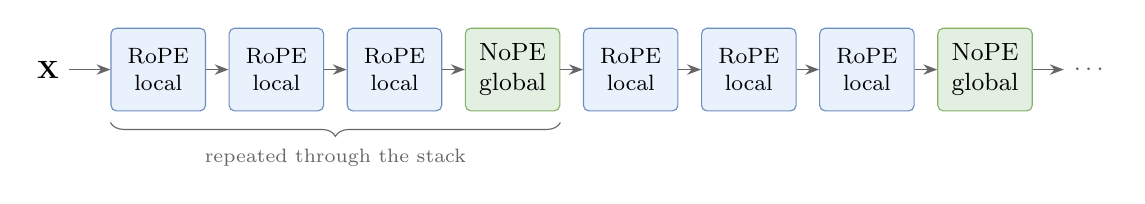
\begin{tikzpicture}[x=1cm, y=1cm,
            rl/.style={tfblk, minimum width=1.2cm, minimum height=1.05cm, align=center, font=\footnotesize},
            nl/.style={rl, tfnorm, minimum width=1.2cm, minimum height=1.05cm}]
        \node[font=\small] (in) at (-0.3,0) {$\vc{X}$};
        \foreach \i/\kind in {0/r,1/r,2/r,3/n,4/r,5/r,6/r,7/n} {
                \if\kind r
                    \node[rl] (b\i) at ({1.1+\i*1.5},0) {RoPE\\local};
                \else
                    \node[nl] (b\i) at ({1.1+\i*1.5},0) {NoPE\\global};
                \fi
            }
        \draw[tfarr] (in) -- (b0);
        \foreach \i [evaluate=\i as \j using int(\i+1)] in {0,...,6}
        \draw[tfarr] (b\i) -- (b\j);
        \draw[tfarr] (b7) -- ++(1,0) node[right, font=\small] {$\cdots$};
        \draw[decorate, decoration={brace, amplitude=5pt, mirror}, drawgray]
        ([yshift=-4pt]b0.south west) -- ([yshift=-4pt]b3.south east)
        node[midway, below=6pt, tflab] {repeated through the stack};
    \end{tikzpicture}
    \par\vspace{0.6em}
    \justifying

    Recent models combine both, for example three RoPE layers, then one NoPE
    layer, repeated through the stack.

    The RoPE layers handle word order among nearby tokens, often restricted to
    a window of recent tokens\NNDSorNN{ (next lecture)}{}. The NoPE layers retrieve from the
    whole context, with no rotation angle that was never seen in training.
    Examples: Llama 4, Command A, SmolLM3.

    \SlideSource{Yang et al. (2025), \textit{Rope to Nope and back again: A new hybrid attention strategy}.}

\end{frame}

\begin{frame}{Positional embeddings at a glance}

    \small
    \renewcommand{\arraystretch}{1.35}
    \begin{tabular}{@{}p{0.17\textwidth}p{0.2\textwidth}p{0.11\textwidth}p{0.2\textwidth}p{0.24\textwidth}@{}}
        \textbf{Method} & \textbf{Position enters}                 & \textbf{Trained} & \textbf{Longer sequences} & \textbf{Used in}      \\
        \hline
        Learned         & added to $\vc{X}$                        & yes              & no                        & BERT, GPT-2, ViT      \\
        Sinusoidal      & added to $\vc{X}$                        & no               & only in theory            & original transformer  \\
        ALiBi           & bias on the scores                       & no               & yes                       & BLOOM, MPT            \\
        RoPE            & rotation of $\qc{\vc{q}}$, $\kc{\vc{k}}$ & no               & degrades                  & most current LLMs     \\
        NoPE            & causal mask only                         & no               & better than RoPE          & interleaved with RoPE \\
    \end{tabular}

\end{frame}

\subsection{The complete transformer model}

\begin{frame}{Putting everything together}
    \setlength{\parskip}{5pt}

    \vspace{0.5em}
    \centering
    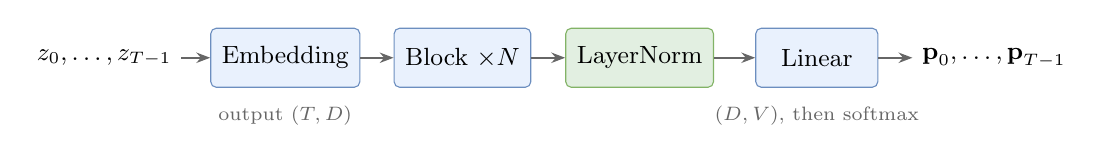
\begin{tikzpicture}[x=1cm, y=1cm]
        \tikzset{pb/.style={tfblk, minimum width=1.55cm}}
        \node[font=\small] (ids) at (0,0) {$z_0,\ldots,z_{T-1}$};
        \node[pb] (emb) at (2.3,0) {Embedding};
        \node[pb] (stack) at (4.55,0) {Block $\times N$};
        \node[pb, tfnorm, minimum width=1.55cm] (ln) at (6.8,0) {LayerNorm};
        \node[pb] (head) at (9.05,0) {Linear};
        \node[font=\small] (out) at (11.3,0) {$\vc{p}_0,\ldots,\vc{p}_{T-1}$};
        \draw[tfarr] (ids) -- (emb);
        \draw[tfarr] (emb) -- (stack);
        \draw[tfarr] (stack) -- (ln);
        \draw[tfarr] (ln) -- (head);
        \draw[tfarr] (head) -- (out);
        \node[tflab, below=3pt] at (emb.south) {output $(T,D)$};
        \node[tflab, below=3pt] at (head.south) {$(D,V)$, then softmax};
    \end{tikzpicture}
    \par\vspace{0.8em}
    \raggedright

    A \myalert{decoder-only} transformer, as in GPT:
    \begin{enumerate}
        \item Embed the tokens (plus positional embeddings, if any).
        \item Apply a stack of $N$ causal transformer blocks.
        \item Apply a final LayerNorm: with pre-norm blocks, the residual path
              is never normalized otherwise.
        \item Apply the same vocabulary classifier at every position.
    \end{enumerate}
    The classifier weights are sometimes shared with the embedding matrix
    (\myalert{weight tying}).

\end{frame}

\begin{frame}{Training and generation}
    \setlength{\parskip}{6pt}

    We train as \NNDSorNN{in the CNN lecture}{at the start of this lecture}, on shifted targets with teacher forcing:
    \[
        \mathcal{L}=-\frac{1}{T}\sum_{t=0}^{T-1}\log\idx{\vc{p}_t}{z_{t+1}} \,.
    \]

    \begin{columns}[T,onlytextwidth]
        \begin{column}{0.49\textwidth}
            \begin{tcolorbox}[nndsgreen,courseheight={tf-traingen}{0.2\textheight}]
                \textbf{\color{darkgreen}Training is parallel}

                One forward pass on $T$ tokens gives all $T$ predictions. The
                causal mask guarantees that $\vc{p}_t$ never sees $z_{t+1}$.
            \end{tcolorbox}
        \end{column}
        \begin{column}{0.49\textwidth}
            \begin{tcolorbox}[nndsorange,courseheight={tf-traingen}{0.2\textheight}]
                \textbf{\color{draworange!70!black}Generation is sequential}

                Each new token needs a forward pass over all the previous
                ones. Caching their keys and values helps\NNDSorNN{ (next lecture)}{}.
            \end{tcolorbox}
        \end{column}
    \end{columns}

    \medskip
    Cheap training and expensive generation drive much of the design of modern
    models.

\end{frame}

\begin{frame}{The residual stream}
    \setlength{\parskip}{6pt}

    In a pre-norm model, the vector of each token is only ever added to.
    Writing $\vc{x}_t$ for its embedding, the final vector is:
    \[
        \vc{h}_t=\vc{x}_t+\sum_{\ell=1}^{N}\Big(
        \eqnmarkbox[drawblue]{mha}{\operatorname{MHA}_{\ell}}+
        \eqnmarkbox[drawgreen]{mlp}{\operatorname{MLP}_{\ell}}\Big)_t \,,
    \]
    \annotate[yshift=-0.8em]{below,left}{mha}{reads all tokens}
    \annotate[yshift=-0.8em]{below,right}{mlp}{reads token $t$ only}
    \vspace{1.2em}

    We can read the model as one \myalert{residual stream} per token: every
    layer reads the stream through a LayerNorm and writes an update back. The
    MHA layers are the only ones that move information between streams.

    As for ResNets, this view explains why removing a single layer often does
    little damage.

    \SlideSource{Elhage et al. (2021), \textit{A mathematical framework for transformer circuits}, Transformer Circuits Thread.}

\end{frame}

\begin{frame}{Visualizing the residual stream}
    \centering
    \vspace{0.5em}
    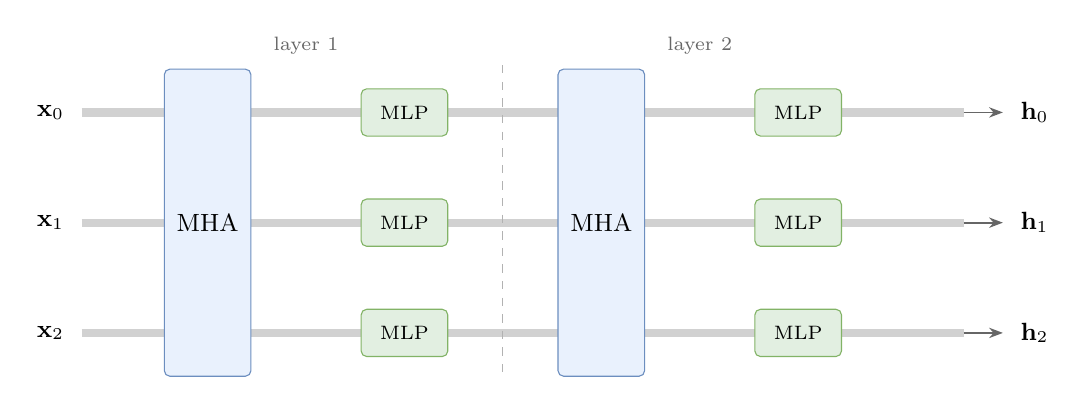
\begin{tikzpicture}[x=1cm, y=1cm,
            stream/.style={line width=3pt, drawgray!30},
            att/.style={tfblk, minimum width=1.1cm, minimum height=3.9cm},
            mlp/.style={tfnorm, minimum width=1.1cm, minimum height=0.6cm, font=\scriptsize},
        ]
        \foreach \y/\t in {0/0,-1.4/1,-2.8/2} {
                \draw[stream] (0.4,\y) -- (11.6,\y);
                \draw[tfarr] (11.6,\y) -- (12.1,\y);
                \node[font=\small, anchor=east] at (0.3,\y) {$\vc{x}_{\t}$};
                \node[font=\small, anchor=west] at (12.2,\y) {$\vc{h}_{\t}$};
                \node[mlp] at (4.5,\y) {MLP};
                \node[mlp] at (9.5,\y) {MLP};
            }
        \node[att] at (2,-1.4) {MHA};
        \node[att] at (7,-1.4) {MHA};
        \node[tflab] at (3.25,0.85) {layer 1};
        \node[tflab] at (8.25,0.85) {layer 2};
        \draw[drawgray!50, dashed] (5.75,0.6) -- (5.75,-3.4);
    \end{tikzpicture}

    \vspace{1.2em}
    {\small Each token has its own stream (gray), from its embedding to the
        output. An MHA layer reads from all the streams and writes to each of
        them; an MLP reads and writes a single stream.\par}

\end{frame}

\begin{frame}{Attention in a trained model}
    \centering
    % Written by scripts/make_gpt2_attention.py: GPT-2 small on "The cat sat on the mat because it was tired.".
% previous: layer 4, head 11
\def\gptheadprevious{layer 4, head 11}
\def\gptcellsprevious{%
\fill[black!100] (0,-0) rectangle ++(1,-1);%
\fill[black!100] (0,-1) rectangle ++(1,-1);%
\fill[black!0] (1,-1) rectangle ++(1,-1);%
\fill[black!0] (0,-2) rectangle ++(1,-1);%
\fill[black!100] (1,-2) rectangle ++(1,-1);%
\fill[black!0] (2,-2) rectangle ++(1,-1);%
\fill[black!0] (0,-3) rectangle ++(1,-1);%
\fill[black!0] (1,-3) rectangle ++(1,-1);%
\fill[black!100] (2,-3) rectangle ++(1,-1);%
\fill[black!0] (3,-3) rectangle ++(1,-1);%
\fill[black!0] (0,-4) rectangle ++(1,-1);%
\fill[black!0] (1,-4) rectangle ++(1,-1);%
\fill[black!0] (2,-4) rectangle ++(1,-1);%
\fill[black!100] (3,-4) rectangle ++(1,-1);%
\fill[black!0] (4,-4) rectangle ++(1,-1);%
\fill[black!0] (0,-5) rectangle ++(1,-1);%
\fill[black!0] (1,-5) rectangle ++(1,-1);%
\fill[black!0] (2,-5) rectangle ++(1,-1);%
\fill[black!0] (3,-5) rectangle ++(1,-1);%
\fill[black!100] (4,-5) rectangle ++(1,-1);%
\fill[black!0] (5,-5) rectangle ++(1,-1);%
\fill[black!0] (0,-6) rectangle ++(1,-1);%
\fill[black!0] (1,-6) rectangle ++(1,-1);%
\fill[black!0] (2,-6) rectangle ++(1,-1);%
\fill[black!0] (3,-6) rectangle ++(1,-1);%
\fill[black!0] (4,-6) rectangle ++(1,-1);%
\fill[black!100] (5,-6) rectangle ++(1,-1);%
\fill[black!0] (6,-6) rectangle ++(1,-1);%
\fill[black!0] (0,-7) rectangle ++(1,-1);%
\fill[black!0] (1,-7) rectangle ++(1,-1);%
\fill[black!0] (2,-7) rectangle ++(1,-1);%
\fill[black!0] (3,-7) rectangle ++(1,-1);%
\fill[black!0] (4,-7) rectangle ++(1,-1);%
\fill[black!0] (5,-7) rectangle ++(1,-1);%
\fill[black!100] (6,-7) rectangle ++(1,-1);%
\fill[black!0] (7,-7) rectangle ++(1,-1);%
\fill[black!0] (0,-8) rectangle ++(1,-1);%
\fill[black!0] (1,-8) rectangle ++(1,-1);%
\fill[black!0] (2,-8) rectangle ++(1,-1);%
\fill[black!0] (3,-8) rectangle ++(1,-1);%
\fill[black!0] (4,-8) rectangle ++(1,-1);%
\fill[black!0] (5,-8) rectangle ++(1,-1);%
\fill[black!0] (6,-8) rectangle ++(1,-1);%
\fill[black!100] (7,-8) rectangle ++(1,-1);%
\fill[black!0] (8,-8) rectangle ++(1,-1);%
\fill[black!0] (0,-9) rectangle ++(1,-1);%
\fill[black!0] (1,-9) rectangle ++(1,-1);%
\fill[black!0] (2,-9) rectangle ++(1,-1);%
\fill[black!0] (3,-9) rectangle ++(1,-1);%
\fill[black!0] (4,-9) rectangle ++(1,-1);%
\fill[black!0] (5,-9) rectangle ++(1,-1);%
\fill[black!0] (6,-9) rectangle ++(1,-1);%
\fill[black!0] (7,-9) rectangle ++(1,-1);%
\fill[black!100] (8,-9) rectangle ++(1,-1);%
\fill[black!0] (9,-9) rectangle ++(1,-1);%
\fill[black!0] (0,-10) rectangle ++(1,-1);%
\fill[black!0] (1,-10) rectangle ++(1,-1);%
\fill[black!0] (2,-10) rectangle ++(1,-1);%
\fill[black!0] (3,-10) rectangle ++(1,-1);%
\fill[black!0] (4,-10) rectangle ++(1,-1);%
\fill[black!0] (5,-10) rectangle ++(1,-1);%
\fill[black!0] (6,-10) rectangle ++(1,-1);%
\fill[black!0] (7,-10) rectangle ++(1,-1);%
\fill[black!0] (8,-10) rectangle ++(1,-1);%
\fill[black!100] (9,-10) rectangle ++(1,-1);%
\fill[black!0] (10,-10) rectangle ++(1,-1);%
\fill[black!0] (0,-11) rectangle ++(1,-1);%
\fill[black!0] (1,-11) rectangle ++(1,-1);%
\fill[black!0] (2,-11) rectangle ++(1,-1);%
\fill[black!0] (3,-11) rectangle ++(1,-1);%
\fill[black!0] (4,-11) rectangle ++(1,-1);%
\fill[black!0] (5,-11) rectangle ++(1,-1);%
\fill[black!0] (6,-11) rectangle ++(1,-1);%
\fill[black!0] (7,-11) rectangle ++(1,-1);%
\fill[black!0] (8,-11) rectangle ++(1,-1);%
\fill[black!0] (9,-11) rectangle ++(1,-1);%
\fill[black!100] (10,-11) rectangle ++(1,-1);%
\fill[black!0] (11,-11) rectangle ++(1,-1);%
}
% first: layer 5, head 1
\def\gptheadfirst{layer 5, head 1}
\def\gptcellsfirst{%
\fill[black!100] (0,-0) rectangle ++(1,-1);%
\fill[black!100] (0,-1) rectangle ++(1,-1);%
\fill[black!0] (1,-1) rectangle ++(1,-1);%
\fill[black!100] (0,-2) rectangle ++(1,-1);%
\fill[black!0] (1,-2) rectangle ++(1,-1);%
\fill[black!0] (2,-2) rectangle ++(1,-1);%
\fill[black!100] (0,-3) rectangle ++(1,-1);%
\fill[black!0] (1,-3) rectangle ++(1,-1);%
\fill[black!0] (2,-3) rectangle ++(1,-1);%
\fill[black!0] (3,-3) rectangle ++(1,-1);%
\fill[black!100] (0,-4) rectangle ++(1,-1);%
\fill[black!0] (1,-4) rectangle ++(1,-1);%
\fill[black!0] (2,-4) rectangle ++(1,-1);%
\fill[black!0] (3,-4) rectangle ++(1,-1);%
\fill[black!0] (4,-4) rectangle ++(1,-1);%
\fill[black!100] (0,-5) rectangle ++(1,-1);%
\fill[black!0] (1,-5) rectangle ++(1,-1);%
\fill[black!0] (2,-5) rectangle ++(1,-1);%
\fill[black!0] (3,-5) rectangle ++(1,-1);%
\fill[black!0] (4,-5) rectangle ++(1,-1);%
\fill[black!0] (5,-5) rectangle ++(1,-1);%
\fill[black!100] (0,-6) rectangle ++(1,-1);%
\fill[black!0] (1,-6) rectangle ++(1,-1);%
\fill[black!0] (2,-6) rectangle ++(1,-1);%
\fill[black!0] (3,-6) rectangle ++(1,-1);%
\fill[black!0] (4,-6) rectangle ++(1,-1);%
\fill[black!0] (5,-6) rectangle ++(1,-1);%
\fill[black!0] (6,-6) rectangle ++(1,-1);%
\fill[black!100] (0,-7) rectangle ++(1,-1);%
\fill[black!0] (1,-7) rectangle ++(1,-1);%
\fill[black!0] (2,-7) rectangle ++(1,-1);%
\fill[black!0] (3,-7) rectangle ++(1,-1);%
\fill[black!0] (4,-7) rectangle ++(1,-1);%
\fill[black!0] (5,-7) rectangle ++(1,-1);%
\fill[black!0] (6,-7) rectangle ++(1,-1);%
\fill[black!0] (7,-7) rectangle ++(1,-1);%
\fill[black!99] (0,-8) rectangle ++(1,-1);%
\fill[black!0] (1,-8) rectangle ++(1,-1);%
\fill[black!0] (2,-8) rectangle ++(1,-1);%
\fill[black!0] (3,-8) rectangle ++(1,-1);%
\fill[black!0] (4,-8) rectangle ++(1,-1);%
\fill[black!0] (5,-8) rectangle ++(1,-1);%
\fill[black!0] (6,-8) rectangle ++(1,-1);%
\fill[black!0] (7,-8) rectangle ++(1,-1);%
\fill[black!1] (8,-8) rectangle ++(1,-1);%
\fill[black!99] (0,-9) rectangle ++(1,-1);%
\fill[black!0] (1,-9) rectangle ++(1,-1);%
\fill[black!0] (2,-9) rectangle ++(1,-1);%
\fill[black!0] (3,-9) rectangle ++(1,-1);%
\fill[black!0] (4,-9) rectangle ++(1,-1);%
\fill[black!0] (5,-9) rectangle ++(1,-1);%
\fill[black!0] (6,-9) rectangle ++(1,-1);%
\fill[black!0] (7,-9) rectangle ++(1,-1);%
\fill[black!0] (8,-9) rectangle ++(1,-1);%
\fill[black!0] (9,-9) rectangle ++(1,-1);%
\fill[black!100] (0,-10) rectangle ++(1,-1);%
\fill[black!0] (1,-10) rectangle ++(1,-1);%
\fill[black!0] (2,-10) rectangle ++(1,-1);%
\fill[black!0] (3,-10) rectangle ++(1,-1);%
\fill[black!0] (4,-10) rectangle ++(1,-1);%
\fill[black!0] (5,-10) rectangle ++(1,-1);%
\fill[black!0] (6,-10) rectangle ++(1,-1);%
\fill[black!0] (7,-10) rectangle ++(1,-1);%
\fill[black!0] (8,-10) rectangle ++(1,-1);%
\fill[black!0] (9,-10) rectangle ++(1,-1);%
\fill[black!0] (10,-10) rectangle ++(1,-1);%
\fill[black!100] (0,-11) rectangle ++(1,-1);%
\fill[black!0] (1,-11) rectangle ++(1,-1);%
\fill[black!0] (2,-11) rectangle ++(1,-1);%
\fill[black!0] (3,-11) rectangle ++(1,-1);%
\fill[black!0] (4,-11) rectangle ++(1,-1);%
\fill[black!0] (5,-11) rectangle ++(1,-1);%
\fill[black!0] (6,-11) rectangle ++(1,-1);%
\fill[black!0] (7,-11) rectangle ++(1,-1);%
\fill[black!0] (8,-11) rectangle ++(1,-1);%
\fill[black!0] (9,-11) rectangle ++(1,-1);%
\fill[black!0] (10,-11) rectangle ++(1,-1);%
\fill[black!0] (11,-11) rectangle ++(1,-1);%
}
% it: layer 4, head 3
\def\gptheadit{layer 4, head 3}
\def\gptcellsit{%
\fill[black!100] (0,-0) rectangle ++(1,-1);%
\fill[black!98] (0,-1) rectangle ++(1,-1);%
\fill[black!2] (1,-1) rectangle ++(1,-1);%
\fill[black!82] (0,-2) rectangle ++(1,-1);%
\fill[black!6] (1,-2) rectangle ++(1,-1);%
\fill[black!12] (2,-2) rectangle ++(1,-1);%
\fill[black!2] (0,-3) rectangle ++(1,-1);%
\fill[black!1] (1,-3) rectangle ++(1,-1);%
\fill[black!95] (2,-3) rectangle ++(1,-1);%
\fill[black!2] (3,-3) rectangle ++(1,-1);%
\fill[black!3] (0,-4) rectangle ++(1,-1);%
\fill[black!1] (1,-4) rectangle ++(1,-1);%
\fill[black!90] (2,-4) rectangle ++(1,-1);%
\fill[black!6] (3,-4) rectangle ++(1,-1);%
\fill[black!1] (4,-4) rectangle ++(1,-1);%
\fill[black!13] (0,-5) rectangle ++(1,-1);%
\fill[black!1] (1,-5) rectangle ++(1,-1);%
\fill[black!62] (2,-5) rectangle ++(1,-1);%
\fill[black!19] (3,-5) rectangle ++(1,-1);%
\fill[black!4] (4,-5) rectangle ++(1,-1);%
\fill[black!1] (5,-5) rectangle ++(1,-1);%
\fill[black!34] (0,-6) rectangle ++(1,-1);%
\fill[black!14] (1,-6) rectangle ++(1,-1);%
\fill[black!22] (2,-6) rectangle ++(1,-1);%
\fill[black!12] (3,-6) rectangle ++(1,-1);%
\fill[black!6] (4,-6) rectangle ++(1,-1);%
\fill[black!10] (5,-6) rectangle ++(1,-1);%
\fill[black!2] (6,-6) rectangle ++(1,-1);%
\fill[black!10] (0,-7) rectangle ++(1,-1);%
\fill[black!6] (1,-7) rectangle ++(1,-1);%
\fill[black!42] (2,-7) rectangle ++(1,-1);%
\fill[black!18] (3,-7) rectangle ++(1,-1);%
\fill[black!13] (4,-7) rectangle ++(1,-1);%
\fill[black!4] (5,-7) rectangle ++(1,-1);%
\fill[black!4] (6,-7) rectangle ++(1,-1);%
\fill[black!3] (7,-7) rectangle ++(1,-1);%
\fill[black!4] (0,-8) rectangle ++(1,-1);%
\fill[black!1] (1,-8) rectangle ++(1,-1);%
\fill[black!87] (2,-8) rectangle ++(1,-1);%
\fill[black!2] (3,-8) rectangle ++(1,-1);%
\fill[black!1] (4,-8) rectangle ++(1,-1);%
\fill[black!0] (5,-8) rectangle ++(1,-1);%
\fill[black!2] (6,-8) rectangle ++(1,-1);%
\fill[black!1] (7,-8) rectangle ++(1,-1);%
\fill[black!1] (8,-8) rectangle ++(1,-1);%
\fill[black!12] (0,-9) rectangle ++(1,-1);%
\fill[black!0] (1,-9) rectangle ++(1,-1);%
\fill[black!55] (2,-9) rectangle ++(1,-1);%
\fill[black!3] (3,-9) rectangle ++(1,-1);%
\fill[black!2] (4,-9) rectangle ++(1,-1);%
\fill[black!0] (5,-9) rectangle ++(1,-1);%
\fill[black!8] (6,-9) rectangle ++(1,-1);%
\fill[black!4] (7,-9) rectangle ++(1,-1);%
\fill[black!12] (8,-9) rectangle ++(1,-1);%
\fill[black!3] (9,-9) rectangle ++(1,-1);%
\fill[black!7] (0,-10) rectangle ++(1,-1);%
\fill[black!1] (1,-10) rectangle ++(1,-1);%
\fill[black!46] (2,-10) rectangle ++(1,-1);%
\fill[black!0] (3,-10) rectangle ++(1,-1);%
\fill[black!0] (4,-10) rectangle ++(1,-1);%
\fill[black!0] (5,-10) rectangle ++(1,-1);%
\fill[black!2] (6,-10) rectangle ++(1,-1);%
\fill[black!1] (7,-10) rectangle ++(1,-1);%
\fill[black!35] (8,-10) rectangle ++(1,-1);%
\fill[black!6] (9,-10) rectangle ++(1,-1);%
\fill[black!2] (10,-10) rectangle ++(1,-1);%
\fill[black!15] (0,-11) rectangle ++(1,-1);%
\fill[black!3] (1,-11) rectangle ++(1,-1);%
\fill[black!24] (2,-11) rectangle ++(1,-1);%
\fill[black!4] (3,-11) rectangle ++(1,-1);%
\fill[black!1] (4,-11) rectangle ++(1,-1);%
\fill[black!1] (5,-11) rectangle ++(1,-1);%
\fill[black!3] (6,-11) rectangle ++(1,-1);%
\fill[black!2] (7,-11) rectangle ++(1,-1);%
\fill[black!18] (8,-11) rectangle ++(1,-1);%
\fill[black!6] (9,-11) rectangle ++(1,-1);%
\fill[black!22] (10,-11) rectangle ++(1,-1);%
\fill[black!1] (11,-11) rectangle ++(1,-1);%
}
\def\gpttokens{$\langle$bos$\rangle$,The,cat,sat,on,the,mat,because,it,was,tired,.}

    \vspace{0.2em}
    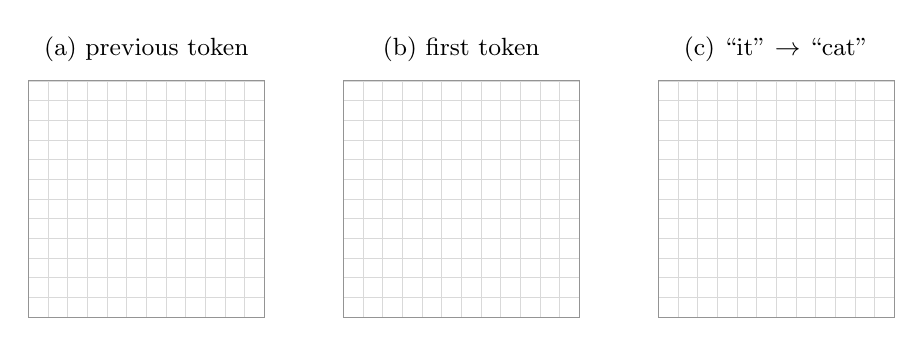
\begin{tikzpicture}[x=0.25cm, y=0.25cm,
            lab/.style={font=\tiny, text=black!70},
            ttl/.style={font=\small},
        ]
        \foreach \name/\x/\title in {previous/0/{(a) previous token}, first/16/{(b) first token}, it/32/{(c) ``it'' $\rightarrow$ ``cat''}} {
        \begin{scope}[xshift=\x*0.25cm]
            \foreach \r in {0,...,11} \foreach \c in {0,...,11}
            \draw[drawgray!25, line width=0.2pt] (\c,-\r) rectangle ++(1,-1);
            \csname gptcells\name\endcsname
            \draw[drawgray!70, line width=0.4pt] (0,0) rectangle (12,-12);
            \node[ttl] at (6,1.6) {\title};
            \node[lab] at (6,0.6) {\csname gpthead\name\endcsname};
            \foreach \t [count=\i from 0] in \gpttokens
            \node[lab, anchor=east, rotate=60] at ({\i+0.5},-12.2) {\t};
        \end{scope}
        }
        \foreach \t [count=\i from 0] in \gpttokens
        \node[lab, anchor=east] at (-0.15,{-\i-0.5}) {\t};
    \end{tikzpicture}

    \vspace{0.2em}
    \justifying
    {\small Three of the 144 heads of GPT-2 (small) on the same sentence (rows
        are queries, darker is larger). Some heads have simple, readable roles:
        (a) attends to the previous token, (b) puts almost all its weight on
        the first token, a way to ``do nothing'' (more on this shortly); in (c), ``it'' attends mostly to ``cat''. Many heads
        have no clear pattern.\par}

\end{frame}

\begin{frame}{Classification with an encoder}
    \setlength{\parskip}{6pt}

    To perform classification or regression with an encoder, we can apply a
    final global pooling on the $T$ tokens and one or more fully-connected
    layers.

    An alternative that is empirically found to work well is the
    \myalert{class token}, an additional \textit{trainable} token
    $\vc{c}\in\mathbb{R}^D$ added to the input matrix:
    \[
        \shape{\vc{X}'}{(T+1,D)}=\begin{bmatrix}\vc{c}^{\top}\\\vc{X}\end{bmatrix},
        \qquad
        \vc{H}=\operatorname{Transformer}(\vc{X}'),
        \qquad
        \vc{y}=\operatorname{softmax}\big(\vc{W}^{\top}\idx{\vc{H}}{0,:}\big) \,.
    \]
    The class token attends to all the others, and its output summarizes the
    sequence for the classifier. In a decoder, the last token is the only one
    that has seen the whole sequence, and plays the same role.

\end{frame}

\begin{frame}{Attention sinks and registers}
    \setlength{\parskip}{6pt}

    The attention weights sum to one, so a head with nothing to retrieve still
    has to look somewhere. Trained transformers put this weight on one
    uninformative token, typically the first one (as in GPT-2 above): an
    \myalert{attention sink}, often with very large activations.

    In vision transformers, a few background patches become sinks and scratch
    space for global information, creating artifacts in the attention maps.

    One fix is to add dedicated tokens, called \myalert{registers}: extra
    trainable tokens added like the class token and discarded at the output. Another fix adds an extra score to each head's
    softmax, fixed at zero (a $+1$ in the denominator) or trainable as in
    gpt-oss, so the weights on the tokens can sum to less than one. Sinks
    matter for long contexts\NNDSorNN{ (next lecture)}{}.

    \SlideSource{Xiao et al. (2024), \textit{Efficient streaming language models with attention sinks}, ICLR; Darcet et al. (2024), \textit{Vision transformers need registers}, ICLR; E. Miller (2023), \textit{Attention is off by one}; OpenAI (2025), \textit{gpt-oss model card}.}

\end{frame}

\begin{frame}{Cross-attention}
    \setlength{\parskip}{6pt}

    Given \textit{two} sequences $\vc{X}\sim(T,D)$ and $\vc{Z}\sim(T',D')$,
    \myalert{cross-attention} takes the queries from the first and the keys and
    values from the second:
    \[
        \shape{\operatorname{CA}(\vc{X},\vc{Z})}{(T,D_v)}
        =\operatorname{softmax}\left(\frac{\qc{(\vc{X}\vc{W}_q)}\kc{(\vc{Z}\vc{W}_k)}^{\top}}{\sqrt{D_k}}\right)\vcl{\vc{Z}\vc{W}_v} \,.
    \]
    The two sequences can have different lengths, and no mask is needed on
    $\vc{Z}$.

    This is a useful operation that can combine information coming from
    different streams of information, e.g., a text and an image, or a text and
    its translation.

\end{frame}

\begin{frame}{Visualizing cross-attention}
    \centering
    \vspace{1em}
    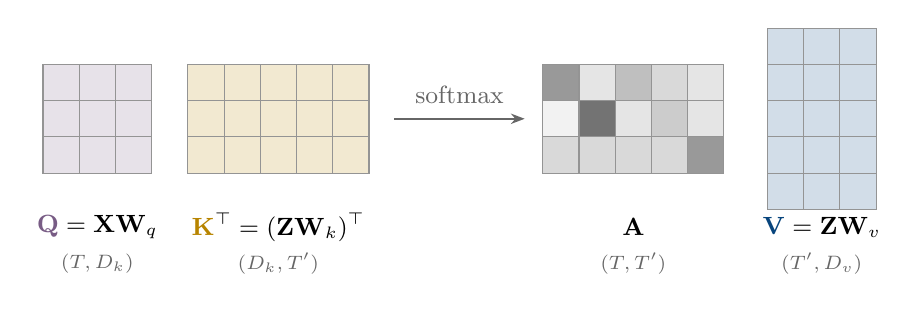
\begin{tikzpicture}[x=0.46cm, y=0.46cm,
            cell/.style={draw=drawgray!70, line width=0.4pt},
            mlab/.style={font=\small},
            slab/.style={font=\scriptsize, text=black!60},
        ]
        % Q from X (T=3 x D_k)
        \foreach \r in {0,...,2} \foreach \c in {0,...,2}
        \draw[cell, fill=qcolor!18] (\c,{-0.5-\r}) rectangle ++(1,-1);
        \node[mlab] at (1.5,-5) {$\qc{\vc{Q}}=\vc{X}\vc{W}_q$};
        \node[slab] at (1.5,-6) {$(T,D_k)$};
        % K^T from Z (D_k x T'=5)
        \foreach \r in {0,...,2} \foreach \c in {0,...,4}
        \draw[cell, fill=kcolor!18] ({4+\c},{-0.5-\r}) rectangle ++(1,-1);
        \node[mlab] at (6.5,-5) {$\kc{\vc{K}}^{\top}=(\vc{Z}\vc{W}_k)^{\top}$};
        \node[slab] at (6.5,-6) {$(D_k,T')$};
        % softmax arrow
        \draw[tfarr] (9.7,-2) -- (13.3,-2)
        node[midway, above=2pt, font=\small] {softmax};
        % A (T x T')
        \def\arow{{40,10,25,15,10},{5,55,10,20,10},{15,15,15,15,40}}
        \foreach \row [count=\r from 0] in \arow {
            \foreach \v [count=\c from 0] in \row {
                \draw[cell, fill=black!\v] ({13.8+\c},{-0.5-\r}) rectangle ++(1,-1);
            }
        }
        \node[mlab] at (16.3,-5) {$\vc{A}$};
        \node[slab] at (16.3,-6) {$(T,T')$};
        % V from Z (T' x D_v)
        \foreach \r in {0,...,4} \foreach \c in {0,...,2}
        \draw[cell, fill=vcolor!18] ({20+\c},{0.5-\r}) rectangle ++(1,-1);
        \node[mlab] at (21.5,-5) {$\vcl{\vc{V}}=\vc{Z}\vc{W}_v$};
        \node[slab] at (21.5,-6) {$(T',D_v)$};
    \end{tikzpicture}

    \vspace{1.5em}
    {\small Each of the $T$ tokens of $\vc{X}$ gets a row of weights over the
        $T'$ tokens of $\vc{Z}$, and collects their values. The attention
        matrix is no longer square.\par}

\end{frame}

\begin{frame}{Encoder-decoder models}
    \centering
    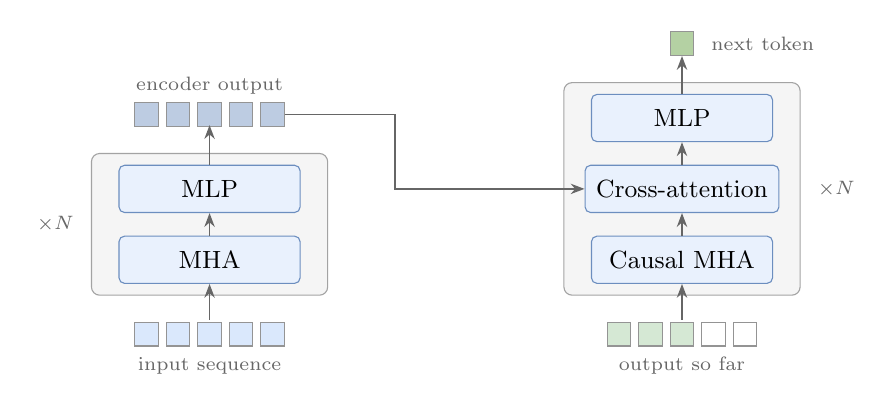
\begin{tikzpicture}[x=1cm, y=0.9cm,
            tok/.style={draw=drawgray!70, minimum size=0.3cm, inner sep=0pt},
            grp/.style={draw=drawgray!60, rounded corners=3pt, fill=drawgray_l},
            sub/.style={tfblk, minimum width=2.3cm, minimum height=0.6cm},
        ]
        % Encoder
        \draw[grp] (-1.5,0.55) rectangle (1.5,2.55);
        \node[sub] (emha) at (0,1.05) {MHA};
        \node[sub] (emlp) at (0,2.05) {MLP};
        \draw[tfarr] (emha) -- (emlp);
        \node[tflab, anchor=east] at (-1.6,1.55) {$\times N$};
        \foreach \i in {0,...,4} {
                \node[tok, fill=drawblue_l] at ({-0.8+\i*0.4},0) {};
                \node[tok, fill=drawblue!45] (eo\i) at ({-0.8+\i*0.4},3.1) {};
            }
        \node[tflab] at (0,-0.45) {input sequence};
        \draw[tfarr] (0,0.2) -- (emha);
        \draw[tfarr] (emlp) -- (0,2.95);
        \node[tflab] at (0,3.5) {encoder output};
        % Decoder
        \draw[grp] (4.5,0.55) rectangle (7.5,3.55);
        \node[sub] (dc) at (6,1.05) {Causal MHA};
        \node[sub] (dx) at (6,2.05) {Cross-attention};
        \node[sub] (dm) at (6,3.05) {MLP};
        \draw[tfarr] (dc) -- (dx);
        \draw[tfarr] (dx) -- (dm);
        \node[tflab, anchor=west] at (7.6,2.05) {$\times N$};
        \foreach \i in {0,...,4}
        \node[tok, fill=\ifnum\i<3 drawgreen_l\else white\fi] at ({5.2+\i*0.4},0) {};
        \node[tflab] at (6,-0.45) {output so far};
        \draw[tfarr] (6,0.2) -- (dc);
        \node[tok, fill=drawgreen!60] (next) at (6,4.1) {};
        \draw[tfarr] (dm) -- (next);
        \node[tflab, anchor=west] at (6.25,4.1) {next token};
        % Encoder output to cross-attention
        \draw[tfarr] (eo4.east) -- ++(1.4,0) |- (dx.west);
    \end{tikzpicture}
    \par\vspace{0.6em}
    \raggedright\setlength{\parskip}{5pt}

    The original transformer was defined for \myalert{sequence to sequence}
    tasks, such as machine translation: every decoder block reads the encoder
    output with cross-attention. Today: T5, Whisper, image generators.

    \SlideSource{Vaswani et al. (2017), \textit{Attention is all you need}, NeurIPS.}

\end{frame}

\subsection{Computational considerations}

\begin{frame}{Convolutions and attention}
    \centering
    \vspace{0.6em}
    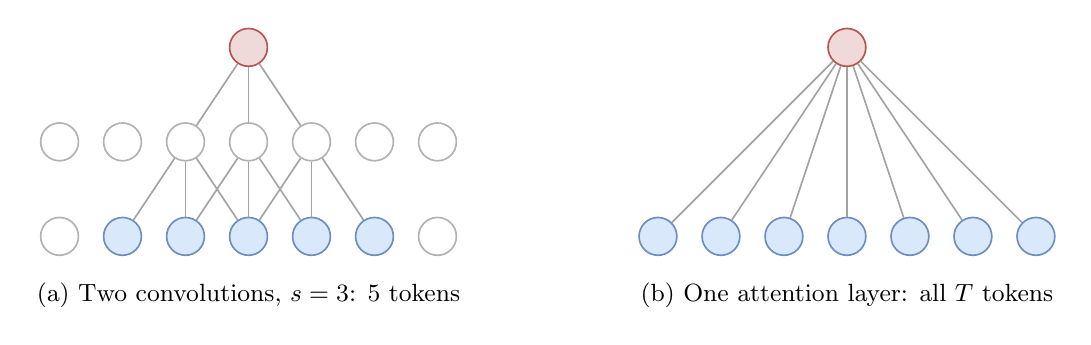
\begin{tikzpicture}[x=0.8cm, y=1cm,
            tok/.style={circle, draw=drawgray!50, fill=white, line width=0.6pt, minimum size=0.48cm, inner sep=0pt},
            seen/.style={tok, draw=drawblue, fill=drawblue_l},
            outt/.style={tok, draw=drawred, fill=drawred!22},
            edge/.style={drawgray!60, line width=0.6pt},
            ptitle/.style={font=\small},
        ]
        % (a) Two convolutional layers with s = 3
        \foreach \i in {0,...,6} {
                \pgfmathtruncatemacro{\inrf}{(\i>=1)&&(\i<=5)}
                \ifnum\inrf=1 \node[seen] (a0\i) at (\i,0) {}; \else \node[tok] (a0\i) at (\i,0) {}; \fi
                \node[tok] (a1\i) at (\i,1.2) {};
            }
        \node[outt] (a2) at (3,2.4) {};
        \foreach \j in {2,3,4} {
                \draw[edge] (a2) -- (a1\j);
                \pgfmathtruncatemacro{\lo}{\j-1}\pgfmathtruncatemacro{\hi}{\j+1}
                \foreach \k in {\lo,...,\hi} \draw[edge] (a1\j) -- (a0\k);
            }
        \node[ptitle] at (3,-0.75) {(a) Two convolutions, $s=3$: 5 tokens};

        % (b) One self-attention layer
        \begin{scope}[xshift=7.6cm]
            \foreach \i in {0,...,6} \node[seen] (b0\i) at (\i,0) {};
            \node[outt] (b1) at (3,2.4) {};
            \foreach \i in {0,...,6} \draw[edge] (b1) -- (b0\i);
            \node[ptitle] at (3,-0.75) {(b) One attention layer: all $T$ tokens};
        \end{scope}
    \end{tikzpicture}

    \vspace{1em}
    \justifying
    {\small After $L$ convolutions with kernel size $s$, an output sees
        $L(s-1)+1$ tokens, and two distant tokens interact only after
        $\mathcal{O}(T/s)$ layers. A single attention layer connects every
        pair of tokens directly, at the price of computing all $T^2$ weights.\NNDSorNN{}{
            In a recurrent model, two tokens at distance $k$ interact through $k$
            sequential state updates.}\par}

\end{frame}

\begin{frame}{Computational cost}
    \setlength{\parskip}{6pt}

    Consider a single layer on $\vc{X}\sim(T,D)$, counting multiply-adds\NNDSorNN{}{. The recurrent
        layer is $\vc{h}_t=\phi(\vc{W}_h\vc{h}_{t-1}+\vc{W}_x\vc{x}_t)$, the convolution has kernel size $s$}:

    \vspace{0.2em}
    \centering
    \renewcommand{\arraystretch}{1.35}
    \NNDSorNN{%
        \begin{tabular}{@{}p{0.26\textwidth}p{0.3\textwidth}p{0.34\textwidth}@{}}
                            & \textbf{Convolution} (kernel $s$) & \textbf{Multi-head attention}         \\
            \hline
            Parameters      & $sD^2$                            & $4D^2$                                \\
            Time            & $\mathcal{O}(TsD^2)$              & $\mathcal{O}(TD^2)+\mathcal{O}(T^2D)$ \\
            Receptive field & $s$ tokens                        & $T$ tokens                            \\
            Extra memory    & none                              & $\vc{A}\sim(T,T)$ per head            \\
        \end{tabular}%
    }{%
        \renewcommand{\arraystretch}{1.2}%
        \begin{tabular}{@{}p{0.2\textwidth}p{0.22\textwidth}p{0.2\textwidth}p{0.3\textwidth}@{}}
                             & \textbf{Recurrent}  & \textbf{Convolution} & \textbf{Multi-head attention}         \\
            \hline
            Parameters       & $2D^2$              & $sD^2$               & $4D^2$                                \\
            Time             & $\mathcal{O}(TD^2)$ & $\mathcal{O}(TsD^2)$ & $\mathcal{O}(TD^2)+\mathcal{O}(T^2D)$ \\
            Sequential steps & $T$                 & $1$                  & $1$                                   \\
            Receptive field  & all past tokens     & $s$ tokens           & $T$ tokens                            \\
            Extra memory     & none                & none                 & $\vc{A}\sim(T,T)$ per head            \\
        \end{tabular}%
    }
    \par\vspace{0.6em}
    \justifying

    The $\mathcal{O}(TD^2)$ term comes from the projections, the
    $\mathcal{O}(T^2D)$ term from $\qc{\vc{Q}}\kc{\vc{K}}^{\top}$ and
    $\vc{A}\vcl{\vc{V}}$. The quadratic term takes over once $T$ is larger
    than (a small multiple of) $D$, which limited early transformers to a few
    hundred tokens.

\end{frame}

\begin{frame}{Where do the parameters go?}
    \setlength{\parskip}{6pt}

    Ignoring biases and normalization, a block with hidden MLP size $4D$ has:
    \[
        \underbrace{4D^2}_{\text{MHA}}+\underbrace{8D^2}_{\text{MLP}}=12D^2
        \text{ parameters.}
    \]
    GPT-2 (small) has $N=12$ blocks, $D=768$ and $V=50{,}257$ tokens:
    \begin{itemize}
        \item blocks: $12\cdot12\cdot768^2\approx 85$M parameters;
        \item token embeddings (tied with the classifier): $V D\approx 39$M;
        \item positional embeddings: $1024\cdot768\approx0.8$M.
    \end{itemize}
    The total is about $124$M. A forward pass costs about $2$ FLOPs per
    parameter and token (one multiply-add), training about three times more.

    \SlideSource{Radford et al. (2019), \textit{Language models are unsupervised multitask learners}; Kaplan et al. (2020), \textit{Scaling laws for neural language models}, arXiv.}

\end{frame}

\begin{frame}{Memory considerations}
    \setlength{\parskip}{6pt}

    Materializing the attention matrices also requires $\mathcal{O}(T^2)$
    memory, for every head and every layer. For example, with $32$ heads,
    $T=32{,}768$ tokens and $16$-bit numbers:
    \[
        32\cdot 32{,}768^2\cdot 2\text{ bytes}\approx 69\text{ GB},
    \]
    for a single layer and a single sequence.

    In practice, $\vc{A}$ is never stored as a whole. Modern implementations
    (e.g., \myalert{FlashAttention}) process the keys in chunks, keeping a
    running maximum and a running denominator of the softmax, and normalize
    only at the end. During generation, the keys and values of past tokens
    are stored in a \myalert{KV cache} instead of being recomputed.\NNDSorNN{

        Both are the starting point of the next lecture.}{}

\end{frame}

\section{Practical transformer models}
\subsection{Text, images and beyond}

\begin{frame}{Transformers everywhere}
    \setlength{\parskip}{6pt}

    Once data is turned into a sequence (or a set) of tokens, the same
    architecture applies almost unchanged:

    \begin{columns}[T,onlytextwidth]
        \begin{column}{0.32\textwidth}
            \begin{tcolorbox}[nndsblue,courseheight={tf-everywhere}{0.36\textheight}]\small
                \textbf{\color{darkcerulean}Audio}\par
                \RaggedRight
                wav2vec 2.0 tokenizes raw audio with a 1D CNN and is
                pre-trained self-supervised; Whisper is an encoder-decoder on
                spectrograms.
            \end{tcolorbox}
        \end{column}
        \begin{column}{0.32\textwidth}
            \begin{tcolorbox}[nndsgreen,courseheight={tf-everywhere}{0.36\textheight}]\small
                \textbf{\color{darkgreen}Graphs}\par
                \RaggedRight
                Nodes become tokens, and the connectivity enters through
                positional embeddings or biases on the scores, as in ALiBi.
            \end{tcolorbox}
        \end{column}
        \begin{column}{0.32\textwidth}
            \begin{tcolorbox}[nndsorange,courseheight={tf-everywhere}{0.36\textheight}]\small
                \textbf{\color{draworange!70!black}Mixer models}\par
                \RaggedRight
                Replacing MHA with an MLP across tokens still works well on
                images: the block structure matters as much as attention.
            \end{tcolorbox}
        \end{column}
    \end{columns}

    \SlideSource{Baevski et al. (2020), \textit{wav2vec 2.0}, NeurIPS; Radford et al. (2023), \textit{Whisper}, ICML; Ying et al. (2021), \textit{Do transformers really perform badly for graph representation?}, NeurIPS; Tolstikhin et al. (2021), \textit{MLP-Mixer}, NeurIPS.}

\end{frame}

\begin{frame}{Transformers for text}
    \setlength{\parskip}{6pt}

    Pre-trained text models differ mostly in the mask and in the objective:

    \begin{columns}[T,onlytextwidth]
        \begin{column}{0.32\textwidth}
            \begin{tcolorbox}[nndsblue,courseheight={tf-text}{0.3\textheight}]\small
                \textbf{\color{darkcerulean}GPT-like (decoders)}\par
                \RaggedRight
                Causal mask, next-token prediction: the model of this lecture.
                Generates one token at a time.
            \end{tcolorbox}
        \end{column}
        \begin{column}{0.32\textwidth}
            \begin{tcolorbox}[nndsgreen,courseheight={tf-text}{0.3\textheight}]\small
                \textbf{\color{darkgreen}BERT-like (encoders)}\par
                \RaggedRight
                No mask; $15\%$ of the tokens are hidden and predicted from
                both sides. For classification and embeddings.
            \end{tcolorbox}
        \end{column}
        \begin{column}{0.32\textwidth}
            \begin{tcolorbox}[nndsorange,courseheight={tf-text}{0.3\textheight}]\small
                \textbf{\color{draworange!70!black}Diffusion LMs}\par
                \RaggedRight
                An encoder starts from a fully hidden sequence and fills it in
                over a few steps, many tokens at once.
            \end{tcolorbox}
        \end{column}
    \end{columns}

    \medskip
    All are \myalert{self-supervised} (the targets come from the text itself)
    and give \myalert{contextual} embeddings: ``bank'' differs in ``river
    bank'' and ``bank account''. Turning them into assistants
    \NNDSorNN{(\textit{post-training}) is the topic of a later lecture}{is called \textit{post-training}}.

    \SlideSource{Devlin et al. (2019), \textit{BERT}, NAACL; Qiu et al. (2020), \textit{Pre-trained models for natural language processing: A survey}; Nie et al. (2025), \textit{Large language diffusion models}, arXiv.}

\end{frame}

\begin{frame}{Applying transformers to images}
    \setlength{\parskip}{6pt}

    Transformers can also be applied in computer vision, especially when
    trained on huge datasets. However, this requires to convert the image (a
    2D grid) into a sequence of tokens.

    Using every pixel as a token is too expensive: a $224\times224$ image has
    about $50{,}000$ pixels, and $50{,}000^2$ attention weights per head. The
    common solution is to work on non-overlapping \myalert{patches}: with
    patches of size $P\times P$, an image $H\times W$ becomes
    \[
        T=\frac{HW}{P^2}\text{ tokens,}
    \]
    each obtained by flattening a patch and projecting it to $D$ features.
    With $P=16$, a $224\times224$ image becomes $14\times14=196$ tokens.

\end{frame}

\begin{whiteframe}{Vision transformer (ViT)}

    \begin{figure}
        \centering
        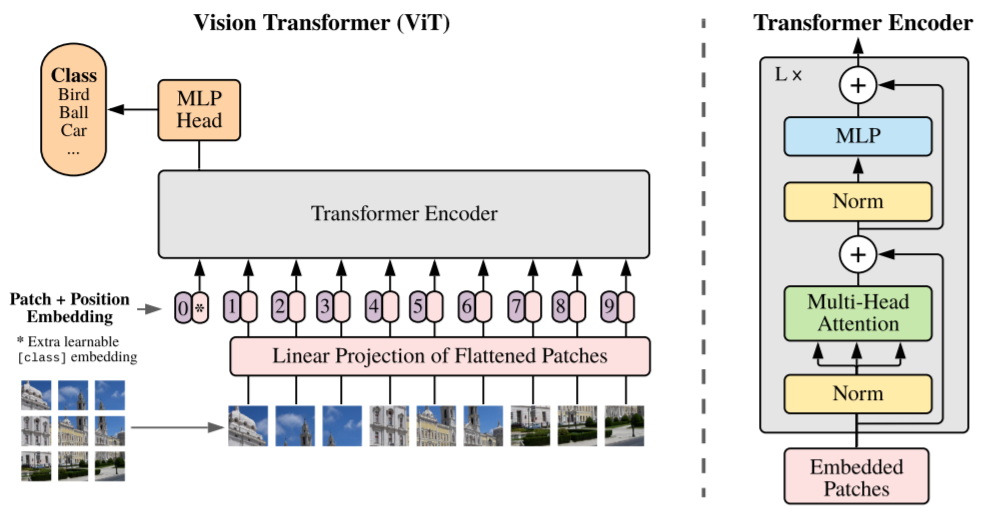
\includegraphics[width=0.7\columnwidth]{images/transformers/2024/VisionTransformer}
    \end{figure}

    {\small The Vision Transformer (ViT) is a standard transformer encoder
    applied on top of image patches, with a class token and trainable
    positional embeddings.\par}

    \SlideSource{Dosovitskiy et al. (2021), \textit{An image is worth 16x16 words: Transformers for image recognition at scale}, ICLR.}

\end{whiteframe}

\begin{frame}[fragile]{Patches as a strided convolution}
    \setlength{\parskip}{6pt}

    Flattening each patch and projecting it with a shared matrix is exactly a
    convolution with kernel size equal to the stride, as in the CNN lecture:

    \begin{python}[gobble=8,aboveskip=4pt,belowskip=4pt]
        patchify = nn.Conv2d(3, D, kernel_size=P, stride=P)
        x = patchify(img)                   # (B, D, H/P, W/P)
        x = x.flatten(2).transpose(1, 2)    # (B, T, D), T = HW/P^2
    \end{python}

    The patch size trades accuracy for cost. Halving $P$ gives $4\times$ more
    tokens and $16\times$ more attention weights: ViT-B/16 and ViT-B/8 have
    the same parameters, but very different costs.

    \SlideSource{Dosovitskiy et al. (2021), \textit{An image is worth 16x16 words: Transformers for image recognition at scale}, ICLR.}

\end{frame}

\begin{frame}{What does a ViT attend to?}
    \centering
    \vspace{0.2em}
    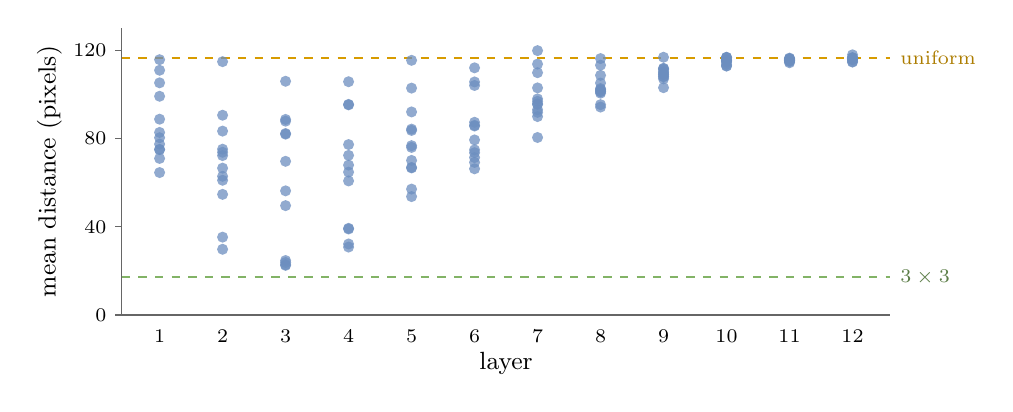
\begin{tikzpicture}[x=0.8cm, y=0.028cm,
            vitdot/.style={fill=drawblue, fill opacity=0.75},
        ]
        \draw[drawgray, line width=0.5pt] (0.4,0) -- (12.6,0);
        \draw[drawgray, line width=0.5pt] (0.4,0) -- (0.4,130);
        \foreach \l in {1,...,12} \node[font=\scriptsize, below=2pt] at (\l,0) {\l};
        \foreach \v in {0,40,80,120} {
                \draw[drawgray] (0.4,\v) -- (0.3,\v);
                \node[font=\scriptsize, left=2pt] at (0.4,\v) {\v};
            }
        \node[font=\small] at (6.5,-22) {layer};
        \node[font=\small, rotate=90] at (-0.75,65) {mean distance (pixels)};
        \draw[draworange, dashed, line width=0.6pt] (0.4,116.5) -- (12.6,116.5)
        node[right, font=\scriptsize, text=draworange!80!black] {uniform};
        \draw[drawgreen, dashed, line width=0.6pt] (0.4,17.2) -- (12.6,17.2)
        node[right, font=\scriptsize, text=drawgreen!70!black] {$3\times3$};
        % Written by attention_distance.py: ViT-B/16 IMAGENET1K_SWAG_LINEAR_V1, 260 Imagenette images.
% Mean attention distance in pixels, one dot per (layer, head).
\fill[vitdot] (1,111.0) circle (2pt);
\fill[vitdot] (1,115.8) circle (2pt);
\fill[vitdot] (1,71.0) circle (2pt);
\fill[vitdot] (1,75.0) circle (2pt);
\fill[vitdot] (1,75.1) circle (2pt);
\fill[vitdot] (1,105.3) circle (2pt);
\fill[vitdot] (1,99.2) circle (2pt);
\fill[vitdot] (1,77.5) circle (2pt);
\fill[vitdot] (1,80.4) circle (2pt);
\fill[vitdot] (1,64.6) circle (2pt);
\fill[vitdot] (1,88.8) circle (2pt);
\fill[vitdot] (1,82.8) circle (2pt);
\fill[vitdot] (2,54.7) circle (2pt);
\fill[vitdot] (2,114.9) circle (2pt);
\fill[vitdot] (2,75.2) circle (2pt);
\fill[vitdot] (2,35.3) circle (2pt);
\fill[vitdot] (2,72.3) circle (2pt);
\fill[vitdot] (2,29.8) circle (2pt);
\fill[vitdot] (2,90.6) circle (2pt);
\fill[vitdot] (2,83.4) circle (2pt);
\fill[vitdot] (2,66.6) circle (2pt);
\fill[vitdot] (2,73.8) circle (2pt);
\fill[vitdot] (2,62.9) circle (2pt);
\fill[vitdot] (2,61.1) circle (2pt);
\fill[vitdot] (3,82.3) circle (2pt);
\fill[vitdot] (3,49.6) circle (2pt);
\fill[vitdot] (3,23.8) circle (2pt);
\fill[vitdot] (3,22.5) circle (2pt);
\fill[vitdot] (3,56.3) circle (2pt);
\fill[vitdot] (3,87.9) circle (2pt);
\fill[vitdot] (3,69.7) circle (2pt);
\fill[vitdot] (3,24.7) circle (2pt);
\fill[vitdot] (3,82.0) circle (2pt);
\fill[vitdot] (3,106.0) circle (2pt);
\fill[vitdot] (3,88.7) circle (2pt);
\fill[vitdot] (3,22.8) circle (2pt);
\fill[vitdot] (4,64.8) circle (2pt);
\fill[vitdot] (4,95.5) circle (2pt);
\fill[vitdot] (4,39.3) circle (2pt);
\fill[vitdot] (4,39.0) circle (2pt);
\fill[vitdot] (4,30.8) circle (2pt);
\fill[vitdot] (4,60.8) circle (2pt);
\fill[vitdot] (4,77.3) circle (2pt);
\fill[vitdot] (4,72.4) circle (2pt);
\fill[vitdot] (4,95.3) circle (2pt);
\fill[vitdot] (4,32.2) circle (2pt);
\fill[vitdot] (4,105.8) circle (2pt);
\fill[vitdot] (4,68.0) circle (2pt);
\fill[vitdot] (5,102.9) circle (2pt);
\fill[vitdot] (5,66.7) circle (2pt);
\fill[vitdot] (5,115.5) circle (2pt);
\fill[vitdot] (5,66.9) circle (2pt);
\fill[vitdot] (5,57.1) circle (2pt);
\fill[vitdot] (5,76.0) circle (2pt);
\fill[vitdot] (5,83.7) circle (2pt);
\fill[vitdot] (5,84.3) circle (2pt);
\fill[vitdot] (5,70.1) circle (2pt);
\fill[vitdot] (5,53.7) circle (2pt);
\fill[vitdot] (5,76.8) circle (2pt);
\fill[vitdot] (5,92.1) circle (2pt);
\fill[vitdot] (6,74.9) circle (2pt);
\fill[vitdot] (6,71.4) circle (2pt);
\fill[vitdot] (6,69.2) circle (2pt);
\fill[vitdot] (6,105.7) circle (2pt);
\fill[vitdot] (6,86.0) circle (2pt);
\fill[vitdot] (6,112.1) circle (2pt);
\fill[vitdot] (6,79.4) circle (2pt);
\fill[vitdot] (6,104.1) circle (2pt);
\fill[vitdot] (6,73.6) circle (2pt);
\fill[vitdot] (6,87.4) circle (2pt);
\fill[vitdot] (6,85.7) circle (2pt);
\fill[vitdot] (6,66.3) circle (2pt);
\fill[vitdot] (7,95.8) circle (2pt);
\fill[vitdot] (7,98.0) circle (2pt);
\fill[vitdot] (7,93.1) circle (2pt);
\fill[vitdot] (7,80.5) circle (2pt);
\fill[vitdot] (7,91.9) circle (2pt);
\fill[vitdot] (7,109.9) circle (2pt);
\fill[vitdot] (7,103.0) circle (2pt);
\fill[vitdot] (7,119.9) circle (2pt);
\fill[vitdot] (7,95.5) circle (2pt);
\fill[vitdot] (7,113.8) circle (2pt);
\fill[vitdot] (7,96.9) circle (2pt);
\fill[vitdot] (7,90.0) circle (2pt);
\fill[vitdot] (8,100.6) circle (2pt);
\fill[vitdot] (8,102.7) circle (2pt);
\fill[vitdot] (8,105.2) circle (2pt);
\fill[vitdot] (8,101.4) circle (2pt);
\fill[vitdot] (8,102.0) circle (2pt);
\fill[vitdot] (8,94.3) circle (2pt);
\fill[vitdot] (8,102.2) circle (2pt);
\fill[vitdot] (8,95.4) circle (2pt);
\fill[vitdot] (8,108.7) circle (2pt);
\fill[vitdot] (8,116.3) circle (2pt);
\fill[vitdot] (8,113.3) circle (2pt);
\fill[vitdot] (8,101.2) circle (2pt);
\fill[vitdot] (9,110.3) circle (2pt);
\fill[vitdot] (9,109.9) circle (2pt);
\fill[vitdot] (9,103.1) circle (2pt);
\fill[vitdot] (9,108.0) circle (2pt);
\fill[vitdot] (9,109.1) circle (2pt);
\fill[vitdot] (9,111.3) circle (2pt);
\fill[vitdot] (9,109.1) circle (2pt);
\fill[vitdot] (9,111.7) circle (2pt);
\fill[vitdot] (9,116.9) circle (2pt);
\fill[vitdot] (9,108.2) circle (2pt);
\fill[vitdot] (9,107.1) circle (2pt);
\fill[vitdot] (9,111.9) circle (2pt);
\fill[vitdot] (10,115.6) circle (2pt);
\fill[vitdot] (10,115.8) circle (2pt);
\fill[vitdot] (10,114.7) circle (2pt);
\fill[vitdot] (10,115.5) circle (2pt);
\fill[vitdot] (10,115.1) circle (2pt);
\fill[vitdot] (10,113.0) circle (2pt);
\fill[vitdot] (10,116.8) circle (2pt);
\fill[vitdot] (10,112.9) circle (2pt);
\fill[vitdot] (10,116.7) circle (2pt);
\fill[vitdot] (10,115.5) circle (2pt);
\fill[vitdot] (10,116.9) circle (2pt);
\fill[vitdot] (10,113.7) circle (2pt);
\fill[vitdot] (11,114.4) circle (2pt);
\fill[vitdot] (11,115.5) circle (2pt);
\fill[vitdot] (11,115.9) circle (2pt);
\fill[vitdot] (11,115.5) circle (2pt);
\fill[vitdot] (11,116.1) circle (2pt);
\fill[vitdot] (11,114.9) circle (2pt);
\fill[vitdot] (11,116.3) circle (2pt);
\fill[vitdot] (11,115.6) circle (2pt);
\fill[vitdot] (11,115.3) circle (2pt);
\fill[vitdot] (11,116.5) circle (2pt);
\fill[vitdot] (11,116.0) circle (2pt);
\fill[vitdot] (11,115.4) circle (2pt);
\fill[vitdot] (12,118.0) circle (2pt);
\fill[vitdot] (12,116.6) circle (2pt);
\fill[vitdot] (12,115.8) circle (2pt);
\fill[vitdot] (12,116.6) circle (2pt);
\fill[vitdot] (12,114.7) circle (2pt);
\fill[vitdot] (12,114.9) circle (2pt);
\fill[vitdot] (12,116.2) circle (2pt);
\fill[vitdot] (12,116.3) circle (2pt);
\fill[vitdot] (12,115.8) circle (2pt);
\fill[vitdot] (12,116.5) circle (2pt);
\fill[vitdot] (12,116.7) circle (2pt);
\fill[vitdot] (12,116.3) circle (2pt);

    \end{tikzpicture}

    \vspace{0.4em}
    \justifying
    {\small Mean distance between a patch and the patches it attends to, one
        dot per head (ViT-B/16 pre-trained on 3.6B images, 260 ImageNet
        images). Middle layers mix local heads with global ones; later layers
        are close to a uniform average. Attention learns part of the locality
        that a convolution hard-codes.\par}

    \SlideSource{As in Dosovitskiy et al. (2021); weights from Singh et al. (2022), CVPR.}

\end{frame}

\begin{frame}{Inductive biases versus data}
    \setlength{\parskip}{6pt}

    Trained only on ImageNet-1k ($1.3$M images), the original ViT is worse than
    a ResNet of similar size. Pre-trained on ImageNet-21k ($14$M) it matches
    it, and on JFT-300M ($300$M) it is better.

    \begin{columns}[T,onlytextwidth]
        \begin{column}{0.49\textwidth}
            \begin{tcolorbox}[nndsblue,courseheight={tf-bias}{0.3\textheight}]
                \textbf{\color{darkcerulean}Better training (DeiT)}

                Strong data augmentation, regularization and distillation from
                a CNN teacher make ViTs competitive on ImageNet-1k alone.
            \end{tcolorbox}
        \end{column}
        \begin{column}{0.49\textwidth}
            \begin{tcolorbox}[nndsgreen,courseheight={tf-bias}{0.3\textheight}]
                \textbf{\color{darkgreen}Better CNNs (ConvNeXt)}

                A ResNet updated with the transformer's design choices and
                training recipe matches vision transformers of similar cost.
            \end{tcolorbox}
        \end{column}
    \end{columns}

    \medskip
    Locality and translation equivariance are useful priors when data is
    scarce; with enough data, attention can learn what it needs.

    \SlideSource{Dosovitskiy et al. (2021), ICLR; Touvron et al. (2021), \textit{Training data-efficient image transformers \& distillation through attention}, ICML; Liu et al. (2022), \textit{A ConvNet for the 2020s}, CVPR.}

\end{frame}

\begin{frame}{Pre-trained vision backbones}
    \setlength{\parskip}{6pt}

    Pre-trained ViTs are today the default image encoders. A name like
    \textit{ViT-B/16} may refer to the architecture or to one of many trained
    versions, shared through hubs (Hugging Face, \texttt{timm},
    \texttt{torchvision}). They differ mostly in how they were trained:

    \begin{itemize}
        \item \textbf{Self-supervised on images}: masked autoencoders (MAE)
              hide $75\%$ of the patches and reconstruct them; DINOv2 and
              DINOv3 train a model to match the features of a slowly updated
              copy of itself. Their patch features work well for dense tasks.
        \item \textbf{Image and text}: CLIP and SigLIP train an image encoder
              and a text encoder so that matching image-caption pairs have
              similar embeddings, enabling zero-shot classification and
              retrieval.
    \end{itemize}

    \SlideSource{He et al. (2022), \textit{Masked autoencoders are scalable vision learners}, CVPR; Oquab et al. (2024), \textit{DINOv2}, TMLR; Siméoni et al. (2025), \textit{DINOv3}, arXiv; Radford et al. (2021), \textit{CLIP}, ICML; Zhai et al. (2023), \textit{SigLIP}, ICCV.}

\end{frame}

\begin{whiteframe}{Multimodal models}

    \begin{figure}
        \centering
        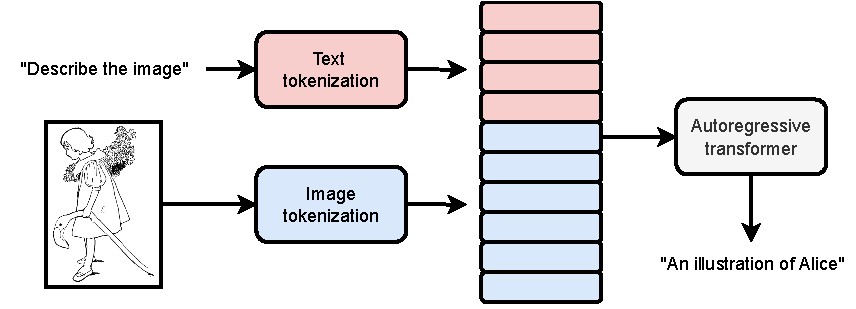
\includegraphics[width=0.75\columnwidth]{images/transformers/book/multimodal_transformer}
    \end{figure}

    {\small Transformers also simplify \myalert{multimodal} models by projecting
    tokens of different modalities in a single embedding space. In most
    vision-language models, the image tokens come from a pre-trained ViT
    (e.g., SigLIP), followed by a small projection.\par}

\end{whiteframe}

\begin{frame}{Further readings}
    \setlength{\parskip}{6pt}

    \begin{itemize}
        \item \textbf{Chapters 10 and 11} \NNDSorNN{from the book}{of \textit{Alice's Adventures in a Differentiable Wonderland}}.
        \item \href{https://jalammar.github.io/illustrated-transformer/}{The Illustrated Transformer}.
        \item \href{https://srush.github.io/raspy/}{Thinking Like Transformers}, for intuitions about how transformers can implement algorithms.
        \item \href{https://transformer-circuits.pub/2021/framework/index.html}{A Mathematical Framework for Transformer Circuits}, for the residual stream view.
    \end{itemize}\NNDSorNN{

        In the next lecture, we go from the 2017 block to a modern language model:
        normalization and MLP variants, the KV cache and how to make it smaller,
        restricted attention, mixtures of experts, and efficient inference.}{}

\end{frame}

\end{document}
